\documentclass[seminar,german]{algothesis}
% possible types: seminar, practical (bachelor, master, zula)
% Für Bachelor-, Master-, und Zulassungsarbeiten die Vorlage my-bachelor-master-zula.tex verwenden!
% possible languages: english, german

\usepackage[utf8]{inputenc}
\usepackage[T1]{fontenc}
\usepackage{lmodern}
\usepackage{amsmath, amssymb, amsthm}
\usepackage{booktabs}
\usepackage{hyperref}
\usepackage{caption}

\usepackage{subcaption}
\usepackage[
    %backend=biber, 
    natbib=true,
    style=numeric,
    sorting=none
]{biblatex}
\addbibresource{mybib.bib}

\graphicspath{{figures/}}
\newcommand*{\quelle}{%
  \footnotesize Quelle:
}


%%%%%%%%%%%%%%%%%%%%%%%%%%%%%%%%%%%%%%%%%%%%%%%%%%%%%%%%%%%%%%%%%%%%%%%%%%
%%%%%%%%%%%%% Bitte nur ab hier Änderungen vornehmen %%%%%%%%%%%%%%%%%%%%%
\title{Sorting Colored Balls in Colored Tubes \\ von Ernst Althaus et. al} % Geben Sie hier den Titel Ihrer Arbeit an.

\author{Philipp Geier} % Geben Sie Ihren Namen an.
\semester{WiSe 2024/25}
\newcommand{\abgabedatum}{28. März 2025} % Hier wird das Abgabedatum angepasst
\supervisors{% Geben Sie die Namen aller Betreuer ab, getrennt durch das Makro '\and'
Jun.-Prof.\ Dr.\ Philipp Kindermann %\and
%Dr.\ Be TreuerInZwei \and
%Be TreuerInDrei, M.\,Sc.
} 


\begin{document}

%%%%%%%%%%%%%%%%%%%%%%%%%%%%%%%%%%%%%%%%%%%%%%%%%%%%%%%%%%%%%%%%%%%%%%%%%%%%%%%%
\setcounter{page}{1}
\section{Einleitung}
In dieser Ausarbeitung geht es um das Thema \glqq Sorting Colored Balls in Colored Tubes \grqq{} von Ernst Althaus et. al. 
\subsection{Bedeutung}
Im Folgenden werden mehrere Wörter und Prinzipien häufig vorkommen, sodass diese zuerst einmal zu erklären sind. Wir schauen uns ein rechteckiges Feld mit Tokens an. Dieses Feld ist in  ein Raster unterteilt und auf jedem Rasterstück kann maximal ein Token platziert werden. Die Position der Tokens kann beliebig aber passend zum Raster gewählt werden. Jede Platzierung nennen wir \textit{\textcolor{blue}{Konfiguration der Tokens}}.  Dabei beschreiben wir das kleinstmögliche Rechteck, das alle Tokens umfasst, als das \textit{\textcolor{blue}{Begrenzungsrechteck}}. Dieses hilft uns bei Verschiebungsoperationen. Diese Operationen sind \textit{\textcolor{blue}{\glqq linepush\grqq{}-Operationen}} in die vier Richtungen ($\Leftarrow, \Uparrow, \Rightarrow, \Downarrow$). 
\\\\
Betrachten wir uns zunächst einen $\Rightarrow$-linepush. Dieser schiebt die Tokens am linken Rand des Begrenzungsrechtecks um eine Einheit im Raster nach rechts. Dabei werden in diese Schieberichtung angrenzende Tokens auch eine Einheit nach rechts verschoben. Abbildung \ref{fig:1} zeigt diesen $\Rightarrow$-linepush. 
\\\\
Der linepush in die weiteren drei Richtungen wird analog jedoch in die jeweilige Richtung ausgeführt.\\
\begin{figure}[ht]
	\centering
	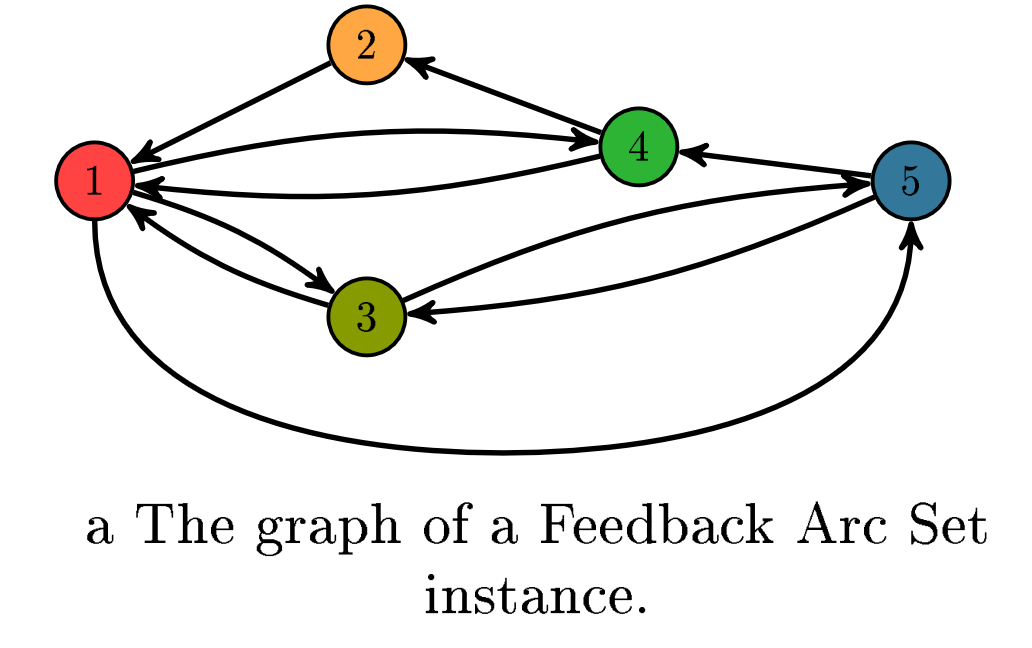
\includegraphics[width=0.8\textwidth]{graph}
	\caption{$\Rightarrow$-linepushes}
	\quelle\cite{akitaya2022pushing}
	\label{fig:1}
\end{figure}

\newpage
\subsection{Anwendung}
Das Konzept vom Manipulieren von Objekten durch uniforme externe Kräfte kommt in mehrere Spielen vor.\\
Beispielsweise kommt das Konzept im Computer-Spiel \glqq 2048\grqq{} vor [Abb. \ref{fig:2}]. Hier gibt es ein quadratisches Feld mit 16 Feldern, auf welchem Tokens drauf sein können. Zu Beginn sind 2 Tokens mit der Aufschrift \glqq 2\grqq{} zufällig auf dem Feld verteilt. Durch Schiebeoperationen verschiebt man alle Tokens in eine Richtung, sodass diese an den Rand oder an Tokens, welche den Rand berühren, angrenzen. Diese Operationen können wir uns als mehrere linepush-Operationen in eine Richtung vorstellen, also so lange einen linepush machen bis die Konfiguration sich nicht mehr verändert. Nach jeder Verschiebung kommt ein weiteres Token mit der Aufschrift \glqq 2\grqq{} oder \glqq 4\grqq{} hinzu. Das besondere an 2048 ist jedoch, dass Tokens mit der selben Nummer beim Verschieben zusammen kommen und die Nummern addiert werden. Gespielt wird bis eine Verschiebung die Konfiguration nicht verändern kann.


\begin{figure}[ht]
	\centering
	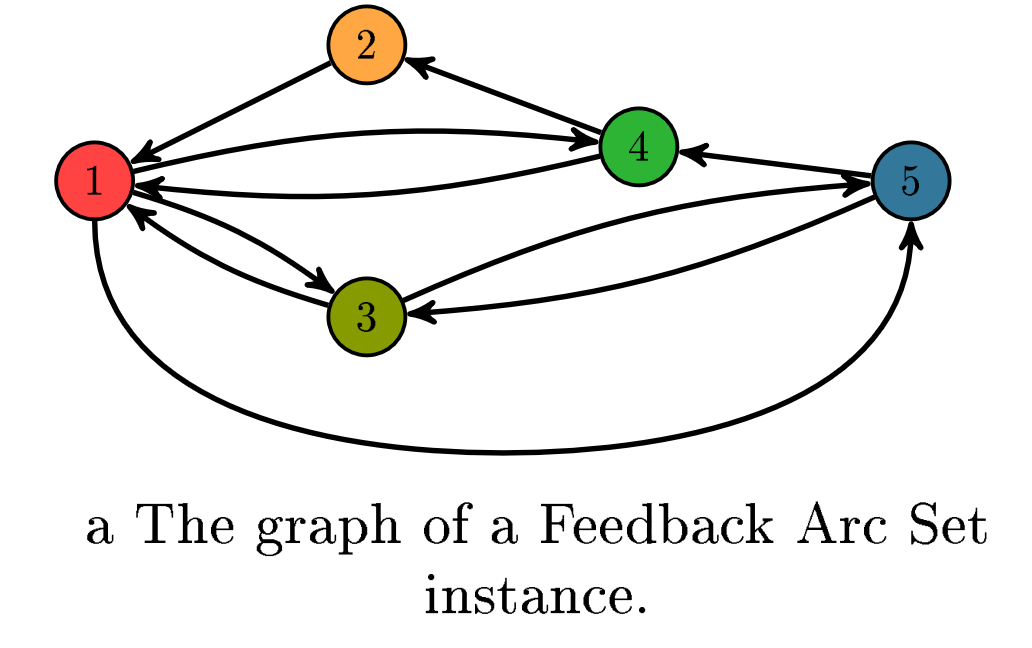
\includegraphics[width=0.25\textwidth]{graph}
	\caption{Spiel 2048}
	\quelle\cite{2048}
	\label{fig:2}
\end{figure}

\noindent
Auch in Geschicklichkeitsspielen wie \glqq Labyrinth\grqq{} [Abb. \ref{fig:lab}] wird das Konzept vom Manipulieren von Objekten genutzt. In diesem Spiel ist die uniforme externe Kraft die Gravitation. Eine Kugel liegt in einem Labyrinth, welches über 2 Räder an den Seiten in unterschiedliche Richtungen geneigt werden kann. Durch die Kombination beider Räder sind nicht nur die Richtungen $\Leftarrow, \Uparrow, \Rightarrow, \Downarrow$ möglich, sondern auch diagonale Richtungen. Durch die Neigung des Feldes fängt die Kugel an zu rollen. Das Ziel des Spieles ist, die Kugel an das Ende des Labyrinths zu führen, ohne dass diese in ein Loch fällt.


\begin{figure}[ht]
	\centering
	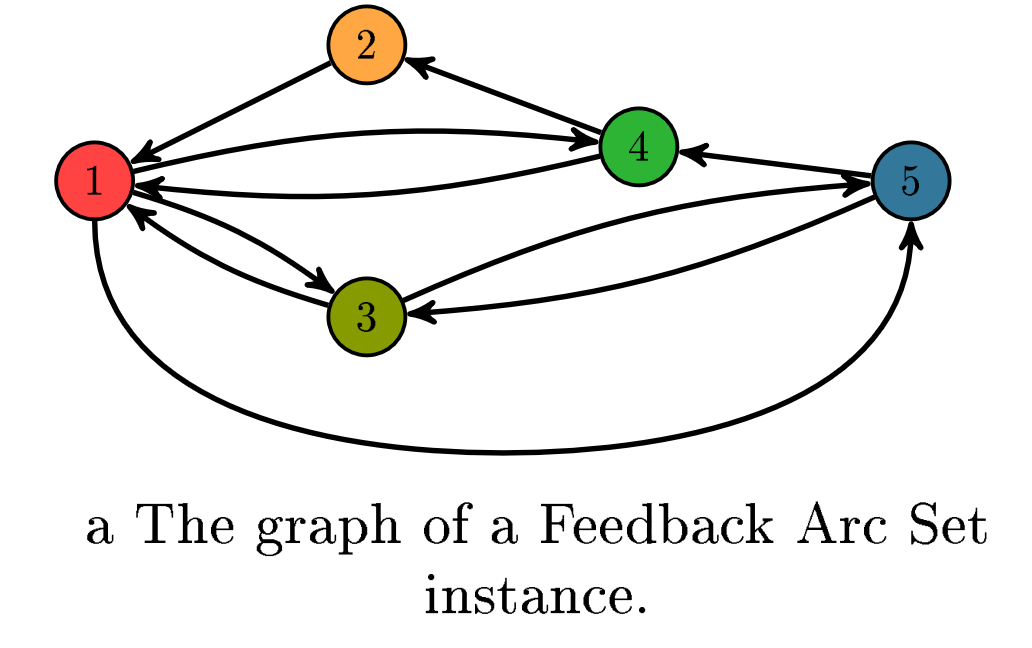
\includegraphics[width=0.29\textwidth]{graph}
	\caption{Geschicklichkeitsspiel Labyrinth}
	\quelle\cite{labyrinth}
	\label{fig:lab}
\end{figure}
\newpage
\noindent
Zum anderen wird das Prinzip für den Selbstzusammenbau und in der robotischen Bewegungsplanung genutzt. Hier wird oftmals mit Teilchen im Micro- und Nanobereich gearbeitet, sodass eine individuelle Bewegung der Teilchen nicht vorstellbar ist. Will man die Teilchen nun bewegen, ist die Herangehensweise mit Hilfe von linepushes sinnvoller, da uniforme externe Kräfte wie ein linepush realisierbar sind.


\section{Puzzle}
Für den weiteren Verlauf der Ausarbeitung sind folgende Definitionen sehr wichtig und werden durchgängig benutzt.

\subsection{Äquivalenz}
\begin{definition}
Zwei Konfigurationen sind äquivalent zueinander, falls die beiden Konfigurationen identisch im Begrenzungsrechteck sind. 
\end{definition}
\noindent Die Konfigurationen werden also bezogen auf das Begrenzungsrechteck betrachtet und bei gleicher Größe des Begrenzungsrechtecks und gleicher Position der Tokens in diesem sind die Konfigurationen äquivalent.


\subsection{Kanonische Konfiguration}
\begin{definition}
Eine Konfiguration heißt kanonisch, falls mehrere $\Rightarrow$-linepushes und \\$\Uparrow$-linepushes eine äquivalente Konfiguration erzeugen.
\end{definition}

\begin{figure}[ht]
	\centering
	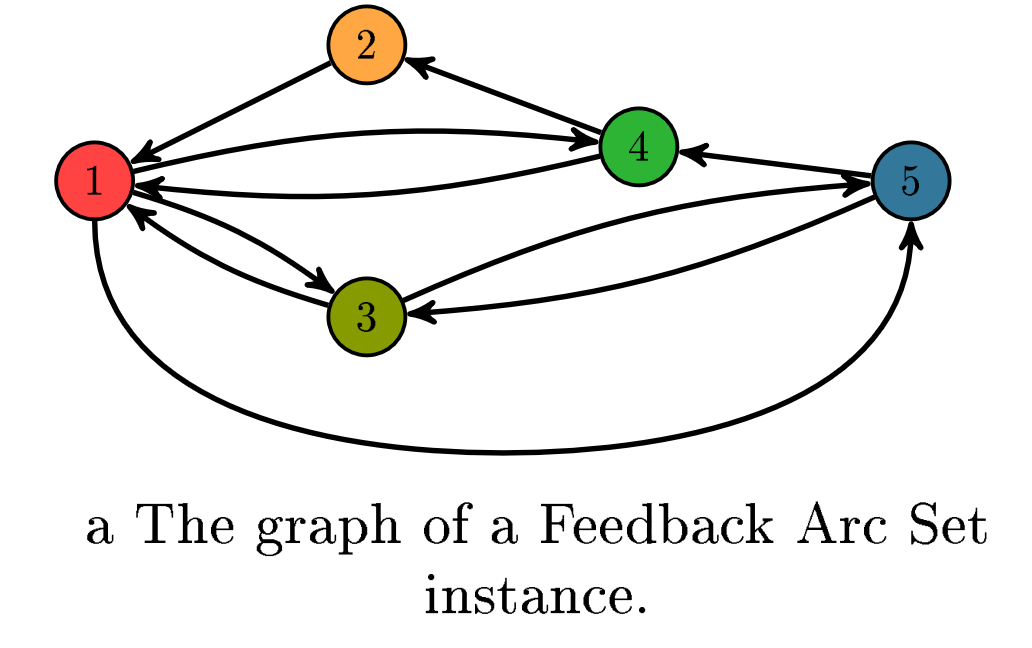
\includegraphics[width=0.25\textwidth]{graph}
	\caption{Kanonische Konfiguration}
	\quelle \cite{akitaya2022pushing}
	\label{fig:3}
\end{figure}

\noindent Eine kanonische Konfiguration ist in Abbildung \ref{fig:3} zu sehen. Hier würde ein $\Rightarrow$-linepush alle Tokens um eine Einheit nach rechts verschieben, da jede Reihe an Tokens an die linke Seite des Begrenzungsrechteck angrenzen und jedes weitere Token unmittelbar von rechts an diese Tokens angrenzt und somit mit nach rechts verschoben werden. Analog ist dies auch für ein $\Uparrow$-linepush und alle Tokens würden um eine Einheit nach oben verschoben werden. Insgesamt bleibt die Konfiguration äquivalent.


\subsection{Kompakte Konfiguration}
\begin{definition}
Eine Konfiguration heißt kompakt, falls ein beliebiger linepush durch einen oder mehrere linepushes rückgängig gemacht werden kann.
\end{definition}
\begin{figure}[ht]
	\centering
	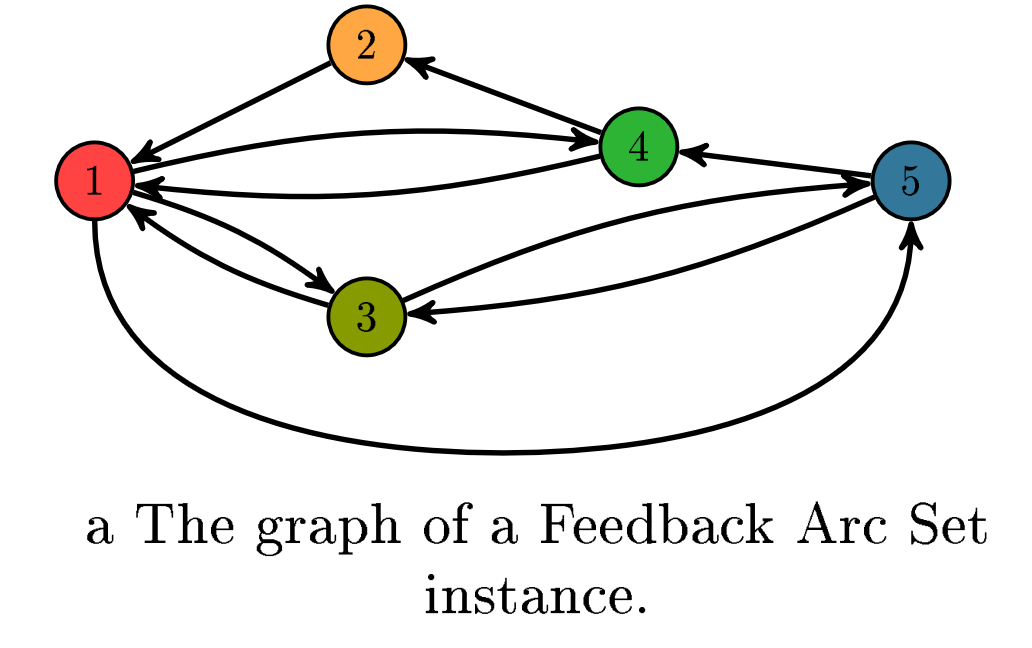
\includegraphics[width=0.25\textwidth]{graph}
	\caption{Kompakte Konfiguration}
	\quelle \cite{akitaya2022pushing}
	\label{fig:4}
\end{figure}
\noindent Ein Beispiel einer kompakten Konfiguration ist in Abbildung \ref{fig:4} abgebildet. Jeder linepush in eine beliebige Richtung kann durch einen oder mehrere linepushes zu einer äquivalenten Konfiguration gemacht werden. \\\\
Schauen wir uns beispielsweise ein $\Leftarrow$-linepush an [Abb. \ref{fig:kmpkt1}]:

\begin{figure}[ht]
	\centering
	\begin{subfigure}{.4\textwidth}
		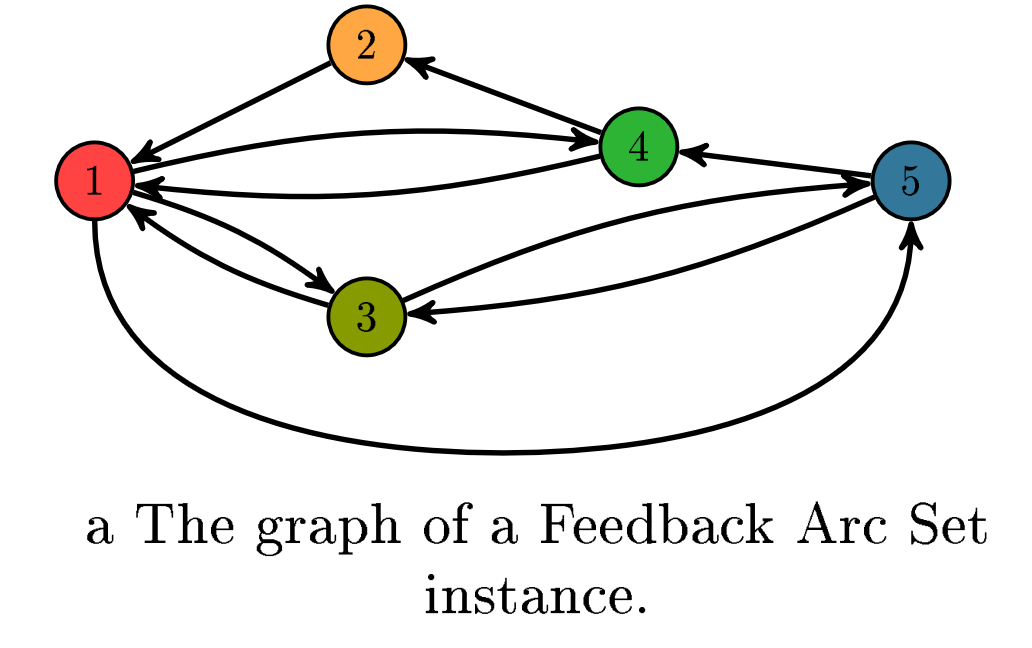
\includegraphics[width=0.78\textwidth]{graph}
    \end{subfigure}%
    \begin{subfigure}{.4\textwidth}
		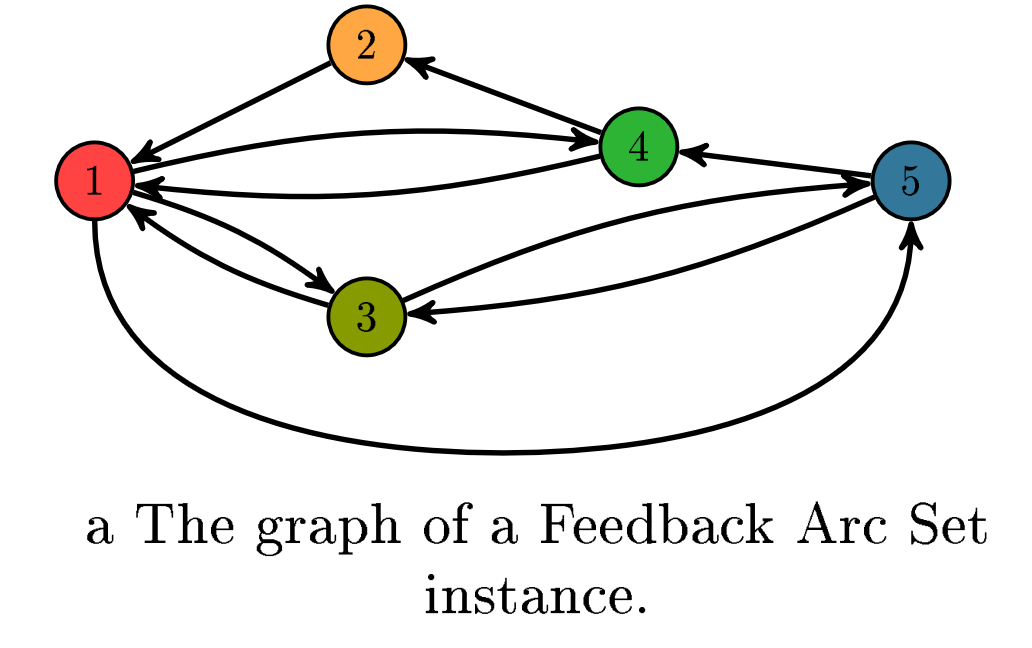
\includegraphics[width=0.78\textwidth]{graph}
    \end{subfigure}
    \caption{$\Leftarrow$-linepush am Beispiel}
    \label{fig:kmpkt1}
\end{figure}

\noindent Um die Ausgangsposition zu erreichen, können wir durch abwechselnde $\Rightarrow$-linepushes und $\Uparrow$-linepushes eine kanonische Konfiguration erzeugen [Abb.\ref{fig:kmpkt2} (links)]. Darauf erreichen wir die Ausgangsposition [Abb.\ref{fig:kmpkt2} (rechts)] mit folgender Sequenz $\langle  \Leftarrow^5~\Downarrow^4 ~\Uparrow\rangle$.

\begin{figure}[ht]
	\centering
	\begin{subfigure}{.4\textwidth}
		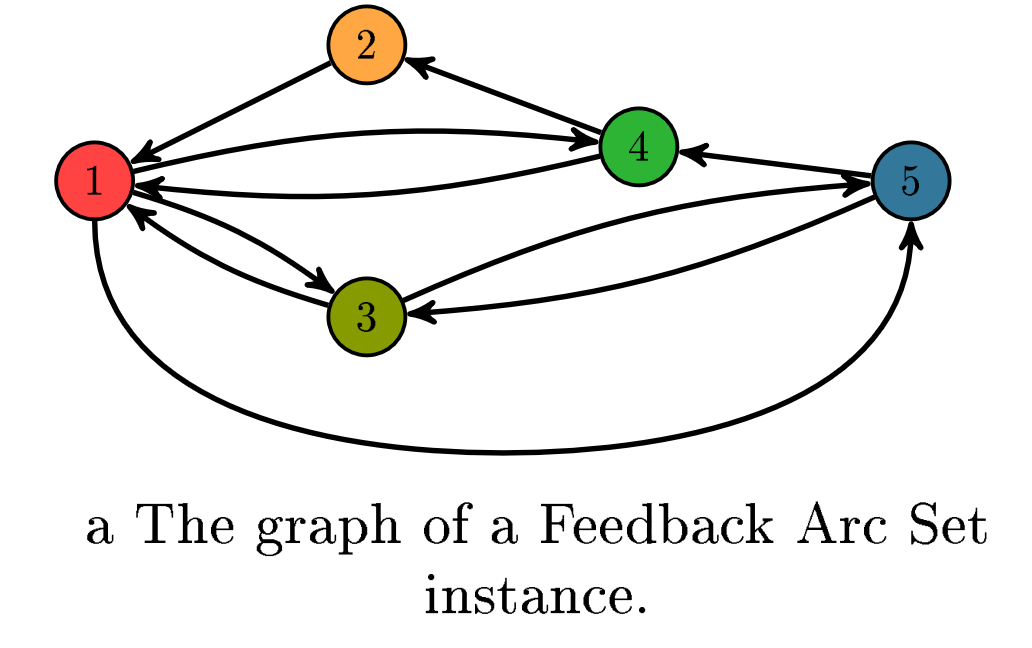
\includegraphics[width=0.78\textwidth]{graph}
    \end{subfigure}%
    \begin{subfigure}{.4\textwidth}
		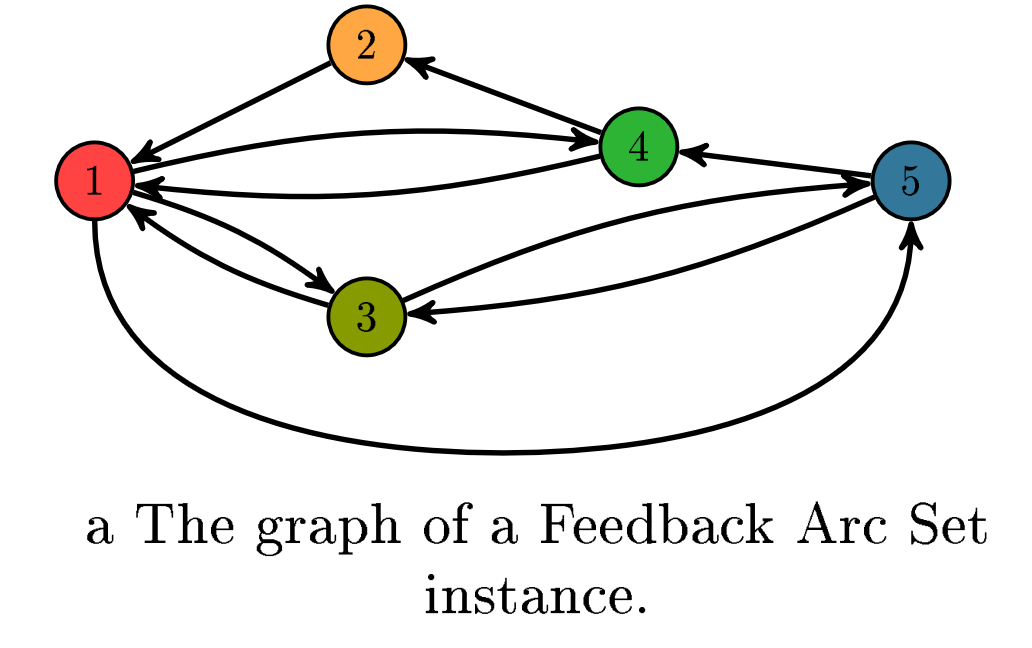
\includegraphics[width=0.78\textwidth]{graph}
    \end{subfigure}
    \caption{Wiederherstellung der Ausgangsposition}
	\label{fig:kmpkt2}
\end{figure}
\newpage
\subsection{Kompatibilität}
\begin{definition}
Zwei Konfigurationen heißen kompatibel, falls die Anzahl von Reihen gleicher Länge in beiden Konfigurationen gleich ist und die Anzahl von Spalten gleicher Länge in beiden Konfigurationen gleich ist.
\end{definition}
\begin{figure}[ht]
	\centering
	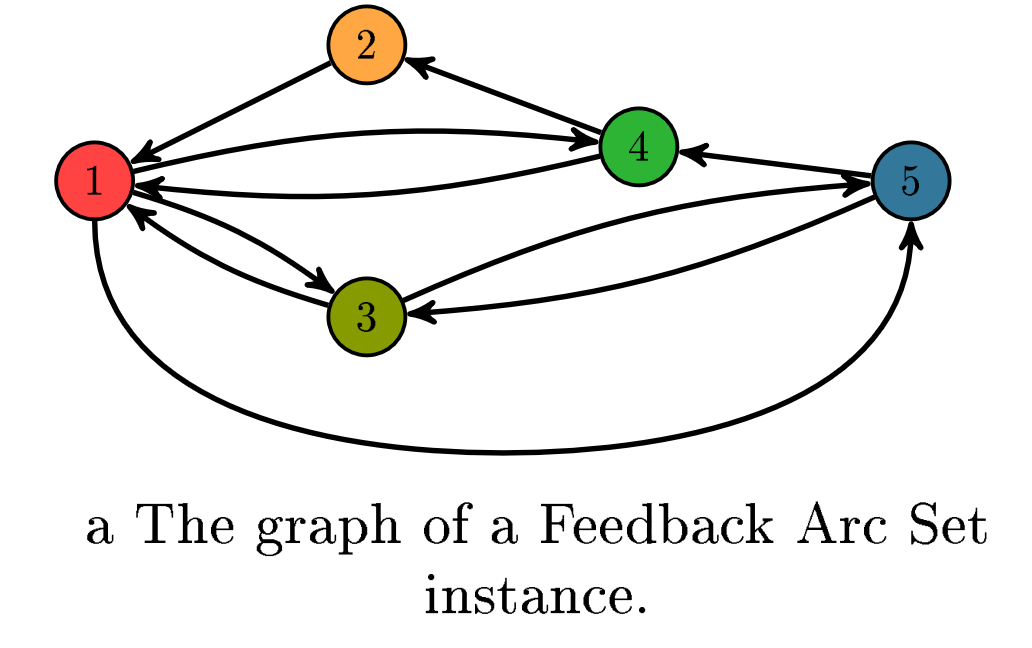
\includegraphics[width=0.5\textwidth]{graph}
	\caption{Kompatibilität von Reihen}
	\quelle \cite{akitaya2022pushing}
	\label{fig:5.1}
\end{figure}
\begin{figure}[ht]
	\centering
	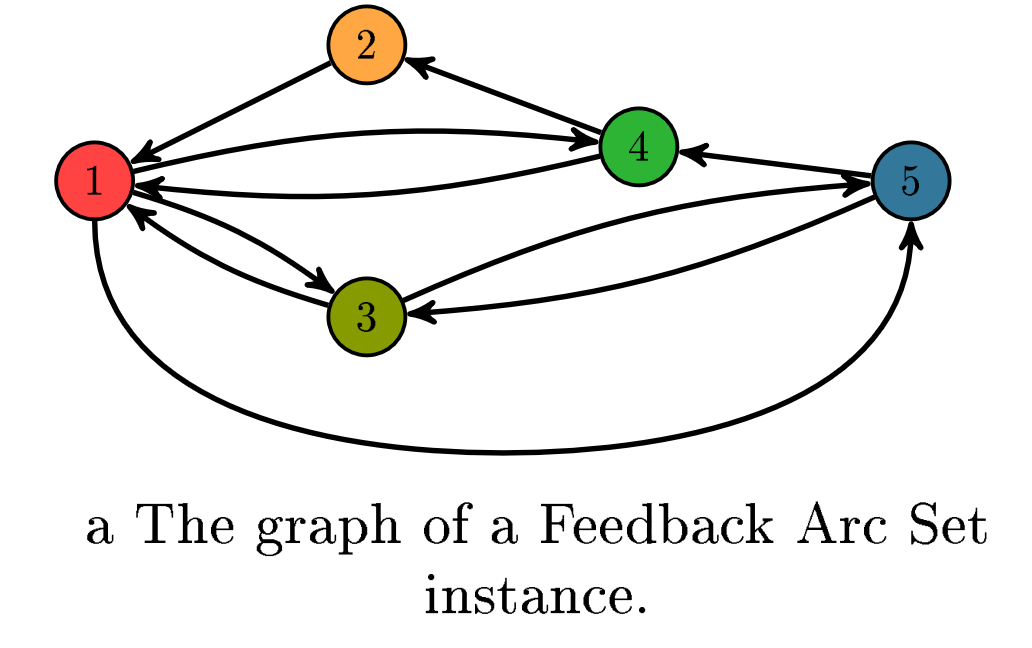
\includegraphics[width=0.5\textwidth]{graph}
	\caption{Kompatibilität von Spalten}
	\quelle \cite{akitaya2022pushing}
	\label{fig:5.2}
\end{figure}

\noindent Die beiden Konfiguration, die in Abbildung \ref{fig:5.1} und Abbildung \ref{fig:5.2} zu sehen sind, sind kompatibel. Denn die Abbildung \ref{fig:5.1} zeigt, dass die Anzahl Reihen gleicher Länge gleich ist und die Abbildung \ref{fig:5.2} zeigt, dass die Anzahl Spalten gleicher Länge gleich ist. Somit sind sie kompatibel.

\subsection{Unbeschriftete/Beschriftete Puzzle}
Wir betrachten uns in dieser Ausarbeitung unbeschriftete und beschriftete Puzzle.\\ Unbeschriftete Puzzle sind Puzzle mit Tokens, die alle entweder keine Beschriftung oder eine einheitliche Beschriftung haben. Hierbei nehmen wir an, dass wir die Tokens dann nicht unterscheiden können. Auch falls Tokens ihre Positionen tauschen wird die Konfiguration als äquivalent bezeichnet. 

\begin{figure}[ht]
	\centering
	\begin{subfigure}{.3\textwidth}
		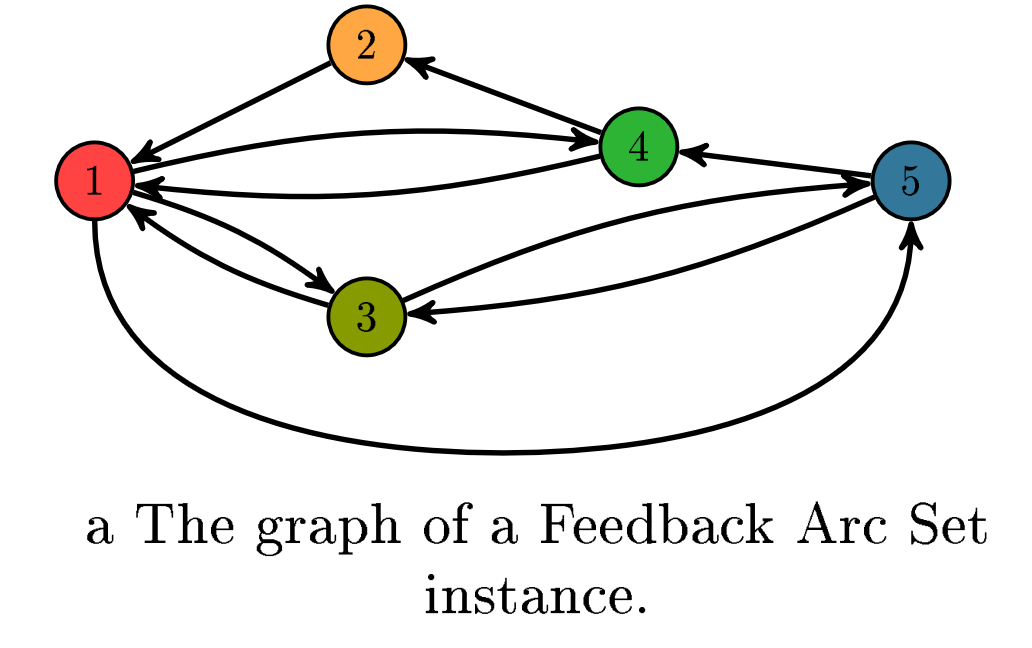
\includegraphics[width=0.75\textwidth]{graph}
    \end{subfigure}%
    \begin{subfigure}{.3\textwidth}
		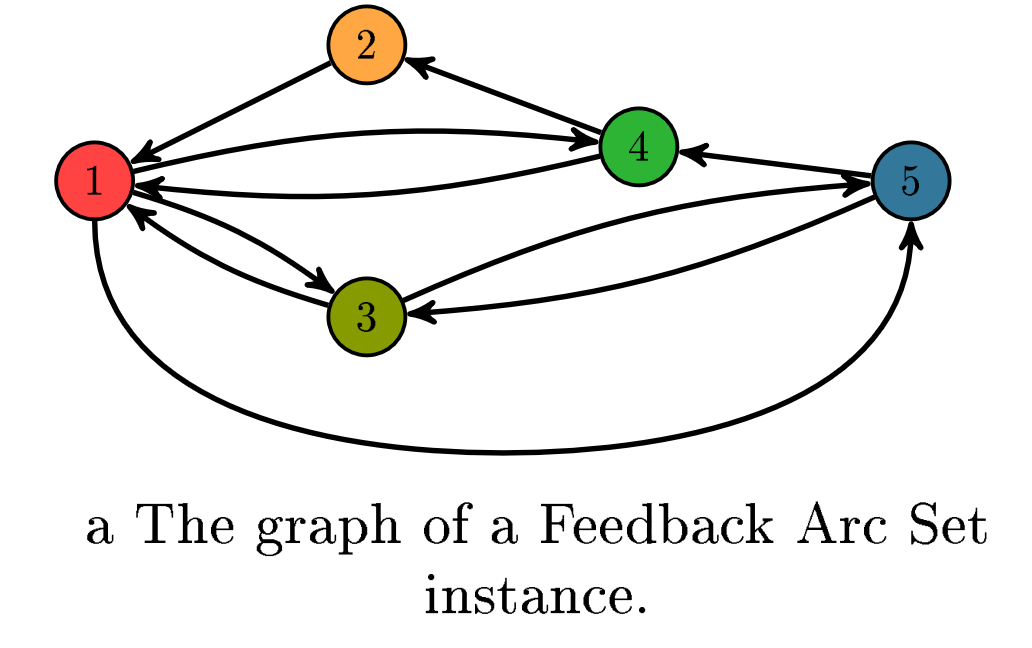
\includegraphics[width=0.7\textwidth]{graph}
    \end{subfigure}
    \caption{Unbeschriftete Konfigurationen}
	\quelle \cite{akitaya2022pushing}
	\label{fig:6}
\end{figure}


\noindent
Beschriftete Puzzle haben eine nicht einheitliche Beschriftung. Die Beschriftung kann über Farben, Zahlen und auch anderweitigen Symbolen erfolgen, solange es mindestens zwei unterschiedliche Beschriftungen sind. Tokens können die selbe Beschriftung zu einem anderen haben, aber werden dann als zueinander äquivalent angesehen. Dies bedeutet, dass die Tokens ohne die Konfiguration zu verändern ausgetauscht werden können. 
\begin{figure}[ht]
	\centering
	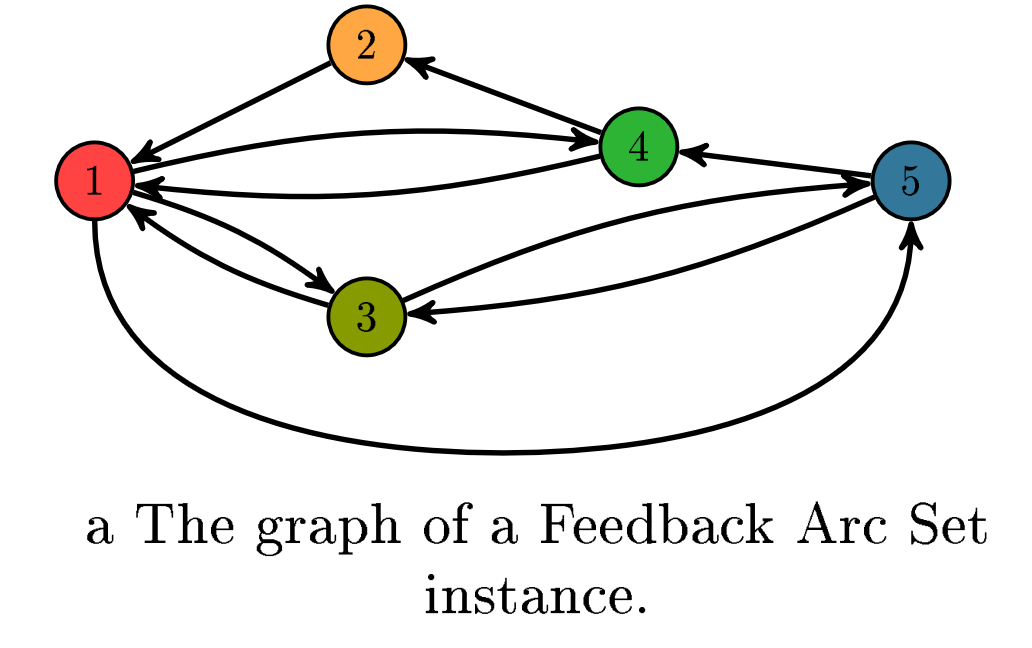
\includegraphics[width=0.23\textwidth]{graph}
	\caption{Beschriftete Konfiguration}
	\quelle \cite{akitaya2022pushing}
	\label{fig:7}
\end{figure}

\section{Verdichtungspuzzle}
Sei eine unbeschriftete verteilte Ausgangskonfiguration gegeben mit $n$ vielen Tokens und $n=ab$. Gibt es eine Folge von linepushes, die eine Konfiguration erzeugt, bei der die Tokens ein $a\times b$ Feld bilden? \\\\
Mit anderen Worten versuchen wir das Begrenzungsrechteck der Anfangskonfiguration auf die Größe $a\times b$ mit Hilfe von linepushes zu verkleinern.

\subsection{Komprimierbare Konfiguration}
\begin{definition}
Eine unbeschriftete Konfiguration heißt komprimierbar, falls ein linepush das Begrenzungsrechteck verkleinern kann.
\end{definition}
\begin{figure}[ht]
	\centering
	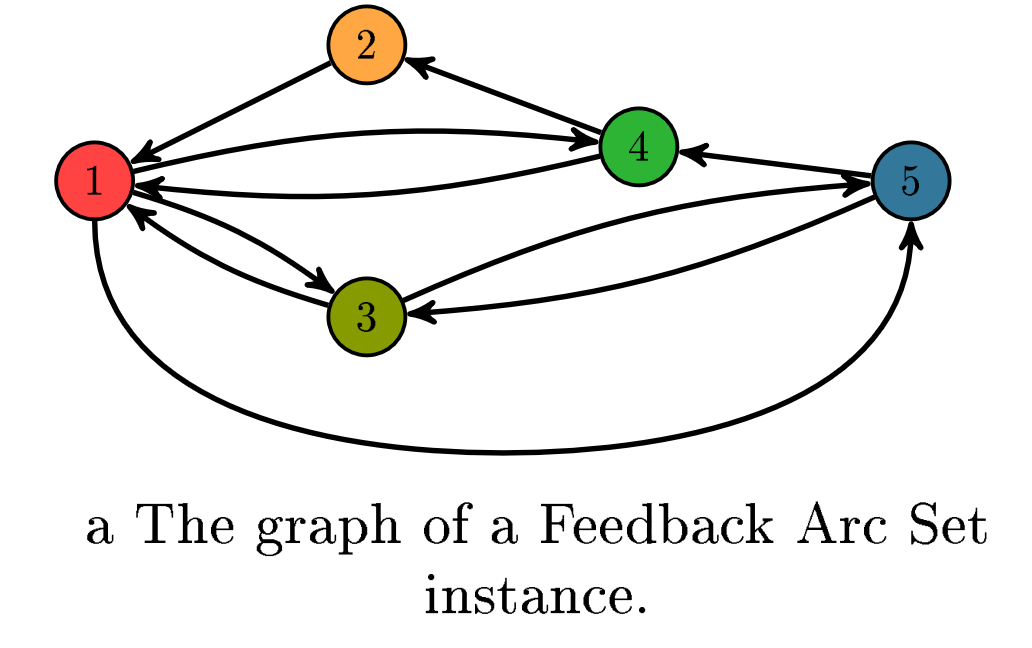
\includegraphics[width=0.23\textwidth]{graph}
	\caption{Komprimierbare Konfiguration}
	\quelle \cite{akitaya2022pushing}
	\label{fig:8}
\end{figure}

\noindent In Abbildung \ref{fig:8} ist eine komprimierbare Konfiguration zu sehen, da das Begrenzungsrechteck der Konfiguration beispielsweise durch einen $\Uparrow$-linepush verkleinert werden kann.

\subsection{Verteilte Konfiguration}
\begin{definition}
Eine unbeschriftete Konfiguration heißt verteilt, falls in jeder Reihe und Spalte maximal ein Token liegt.
\end{definition}
\begin{figure}[ht]
	\centering
	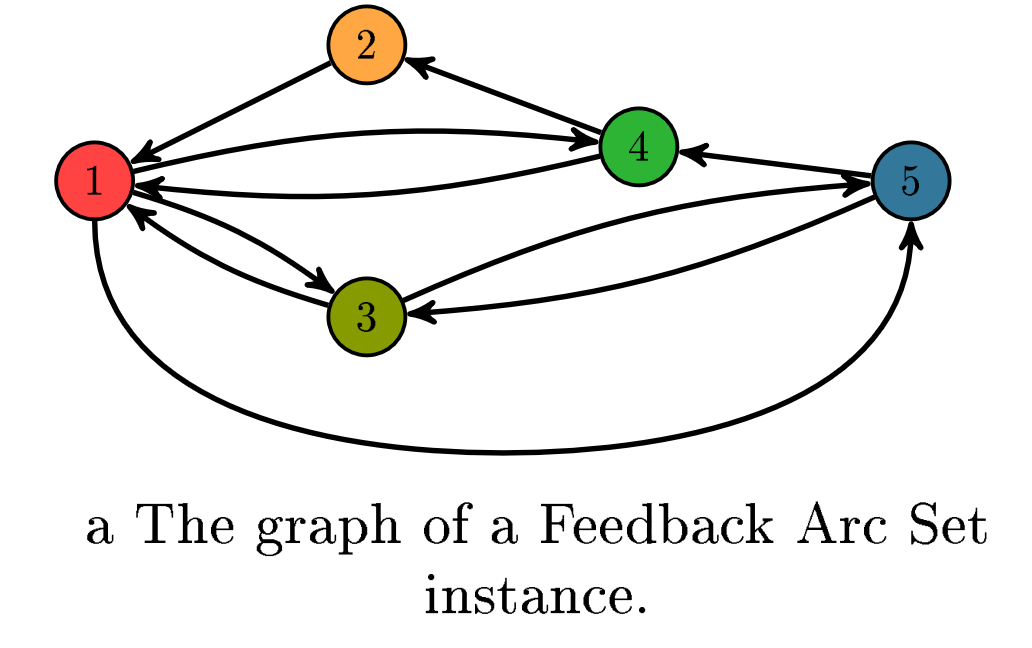
\includegraphics[width=0.23\textwidth]{graph}
	\caption{Verteilte Konfiguration}
	\quelle \cite{akitaya2022pushing}
	\label{fig:9}
\end{figure}
\noindent In Abbildung \ref{fig:9} ist eine verteilte Konfiguration. Jede Reihe hat maximal ein Token und gleichermaßen gilt dies für jede Spalte.
\subsection{Theorem}
Alle verteilten Konfigurationen von $n=a\cdot b$ Tokens mit $a,b\in \mathbb{N}$ kann in eine $a \times b$ Box gedrückt werden, falls und nur falls $a\leq 2$ oder $b\leq 2$ oder $a=b=3$.
\begin{proof}\noindent\\
Da wir von einer verteilten Konfiguration ausgehen, gilt das Theorem für $1\leq a\leq 2$. Weil in jeder Reihe nur maximal ein Token sein kann, können wir $\Uparrow$-linepushes machen bis wir eine Reihe mit $b$ vielen Tokens haben. \\
Falls $a = 2$ führen wir $\Downarrow$-linepushes aus bis wir eine weitere Reihe mit $b$ vielen Tokens haben und diese beide Reihen werden danach mit $\Uparrow$-linepushes oder $\Downarrow$-linepushes zusammengeführt, sodass wir nur noch $a$  viele Reihen haben. Schließlich führen wir $\Rightarrow$-linepushes aus bis unsere Begrenzungsrechteck eine $a\times b$ Box ist. Analog gilt dies für $1\leq b\leq 2$.\\\\
Für $a=b=3$ gehen wir zuerst gleichermaßen vor und erhalten zwei Reihen mit jeweils drei Tokens. Da wir zu Beginn eine verteilte Konfiguration hatten, ist in jeder Spalte maximal ein Token. Dazu sind genau 3 Tokens nicht in der oberen oder unteren Reihe. Dadurch lassen sich die Tokens mit weiteren linepushes zu einer  $3\times 3$ Box zusammenführen. \\\\
Für jedes anderweitige $a$ und $b$ gibt es eine mögliche Startkonfiguration, bei welcher keine $a\times b$ Box durch linepushes entstehen kann:\\

\begin{figure}[ht]
	\centering
	\begin{subfigure}{.3\textwidth}
		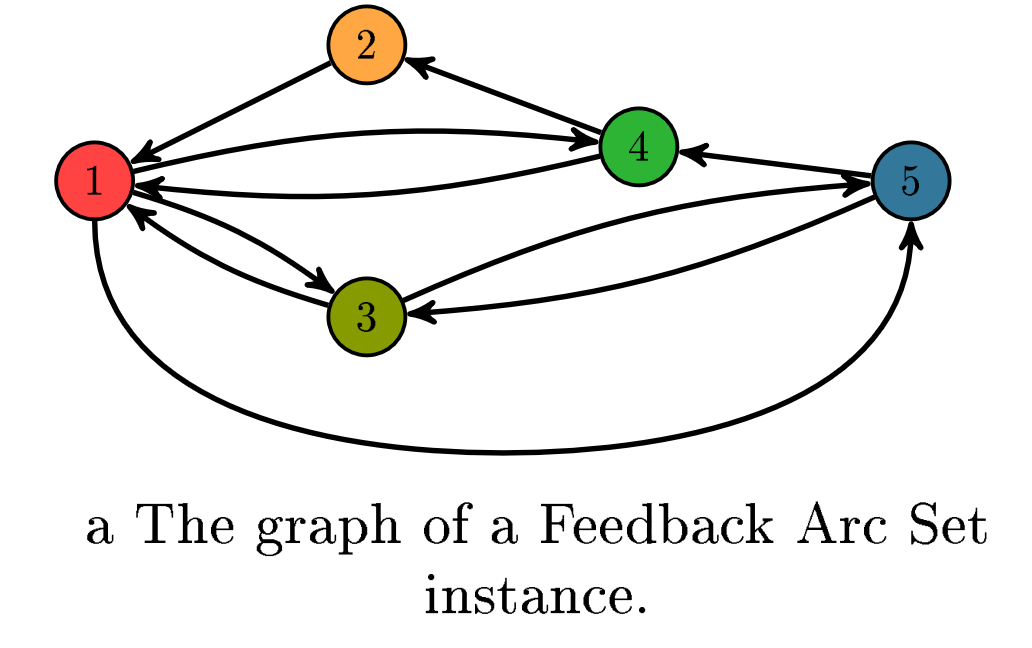
\includegraphics[width=0.73\textwidth]{graph}
		\caption{Start}
    \end{subfigure}%
    \begin{subfigure}{.3\textwidth}
		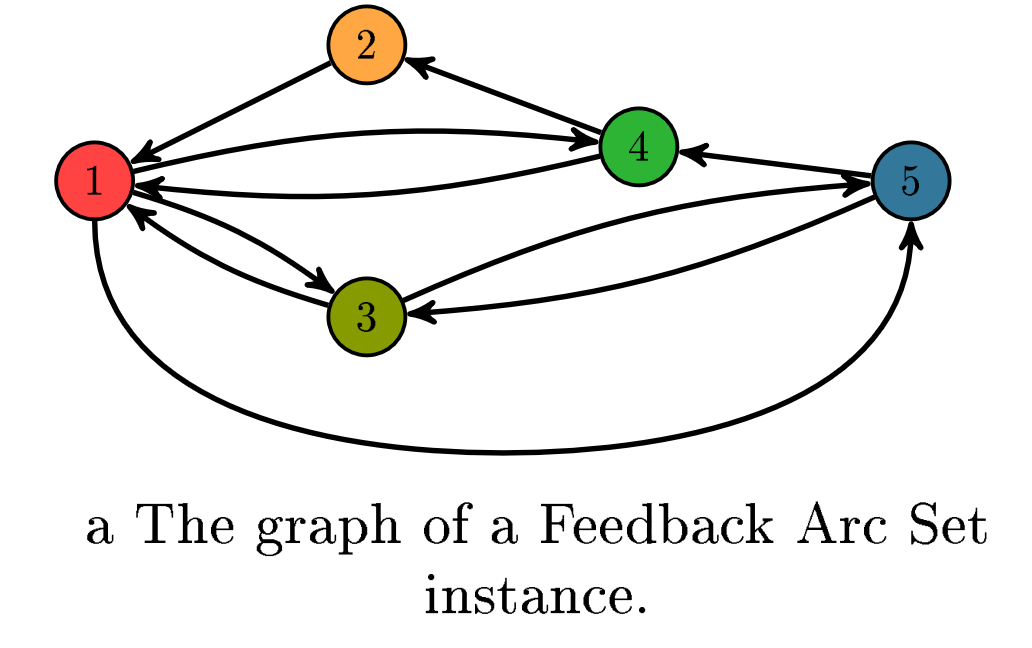
\includegraphics[width=0.65\textwidth]{graph}
		\caption{L-Form}
    \end{subfigure}%
    \begin{subfigure}{.3\textwidth}
		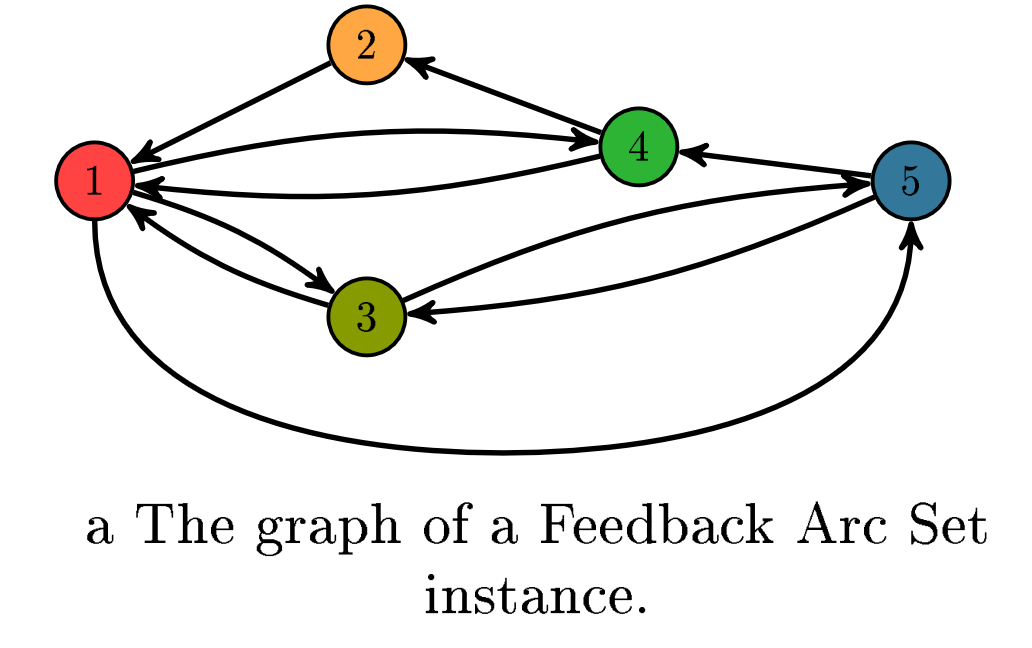
\includegraphics[width=0.35\textwidth]{graph}
		\caption{Ende}
    \end{subfigure}%
    \caption{Ablauf für die doppelte diagonale Ausgangskonfiguration}
	\quelle \cite{akitaya2022pushing}
	\label{fig:13}
\end{figure}

\noindent
Bei dieser Startkonfiguration sind die Tokens in zwei Diagonalen unterteilt wie in Abbildung \ref{fig:13} (a) zu sehen ist. Durch linepushes können wir keine $a\times b$ Box erhalten, da diese L-Formen [Abb. \ref{fig:13} (b)] entstehen, welche $a$ (bzw. $b$) viele Tokens in der Reihe (bzw. Spalte) haben. Dadurch kann die Komprimierung am Ende nicht mehr funktionieren, da mehr als $a$ (bzw. $b$) viele Tokens in der Reihe (bzw. Spalte) sind [Abb. \ref{fig:13} (c)].
\end{proof}

\subsection{Programm}
Um das Verdichtungspuzzle besser zu verstehen, habe ich ein JavaFX Programm geschrieben, um mit diesem linepushes zu simulieren. \\
Auf einer Gridpane werden rote beschriftete Tokens in einem Raster angezeigt und durch das Drücken auf die Knöpfe kann ein linepush in die Richtung des Pfeiles auf den Knöpfen ausgeführt werden.\\
Solange die Konfiguration nicht kompakt ist, kann ein linepush das Begrenzungsrechteck verkleinern. Dieses passt sich automatisch an die Konfiguration an.
\begin{figure}
	\centering
	\begin{subfigure}{.5\textwidth}
		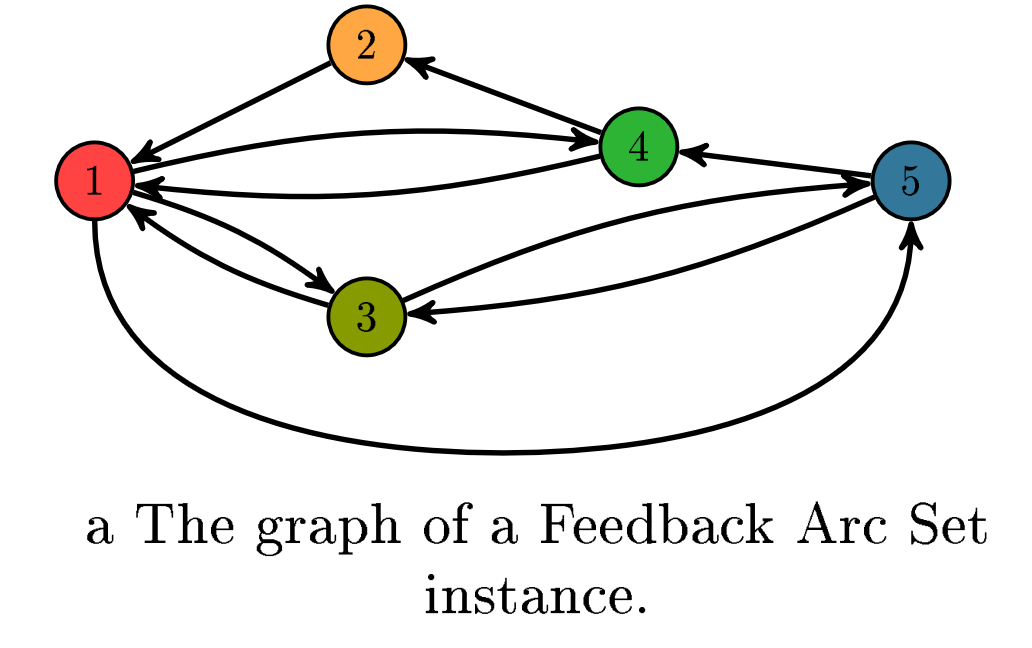
\includegraphics[width=0.75\textwidth]{graph}
    \end{subfigure}%
    \begin{subfigure}{.5\textwidth}
		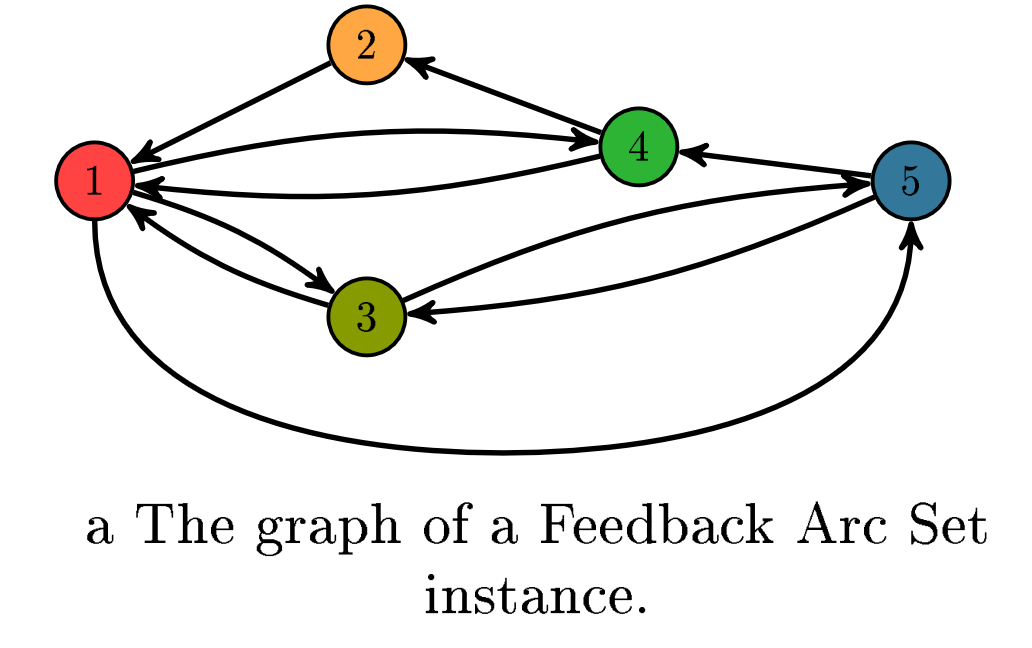
\includegraphics[width=0.75\textwidth]{graph}
    \end{subfigure}
\end{figure}
\begin{figure}
	\centering
	\begin{subfigure}{.5\textwidth}
		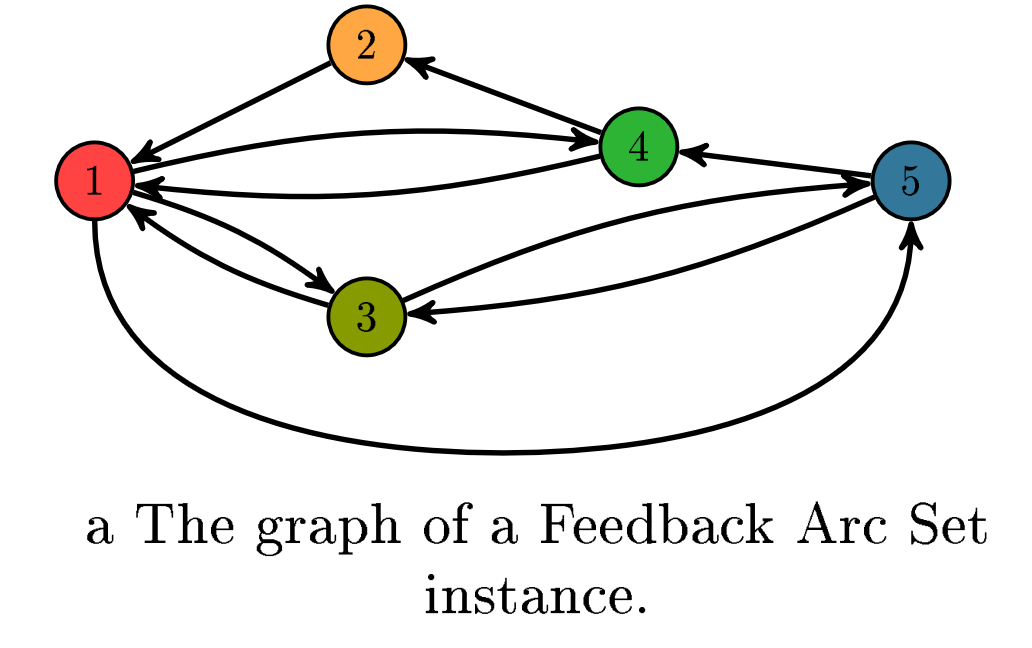
\includegraphics[width=0.75\textwidth]{graph}
    \end{subfigure}%
    \begin{subfigure}{.5\textwidth}
		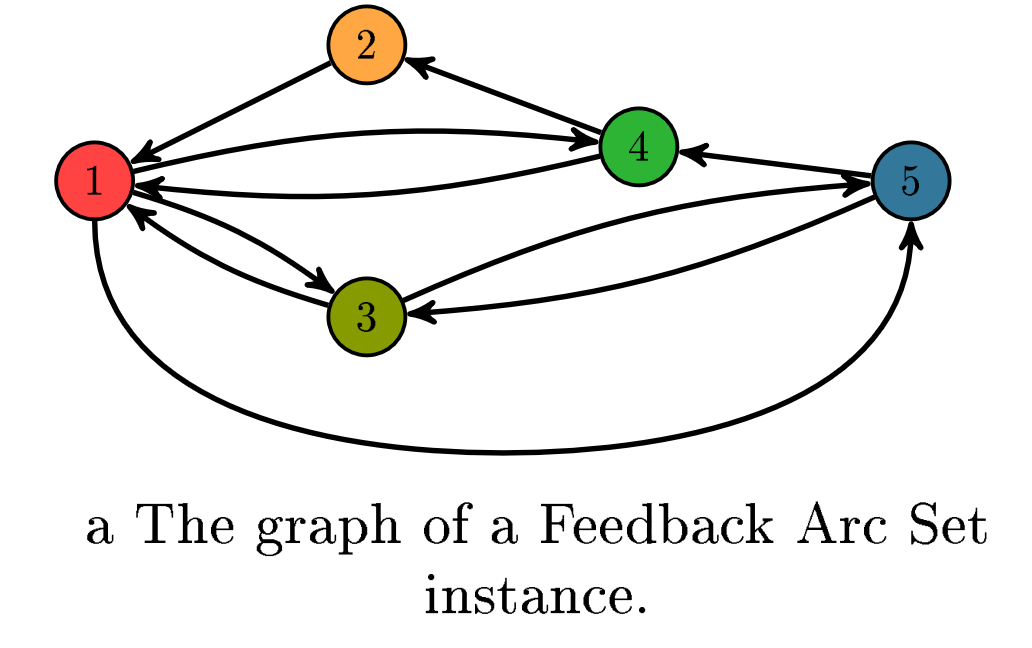
\includegraphics[width=0.75\textwidth]{graph}
    \end{subfigure}
\end{figure}
\begin{figure}
	\centering
	\begin{subfigure}{.5\textwidth}
		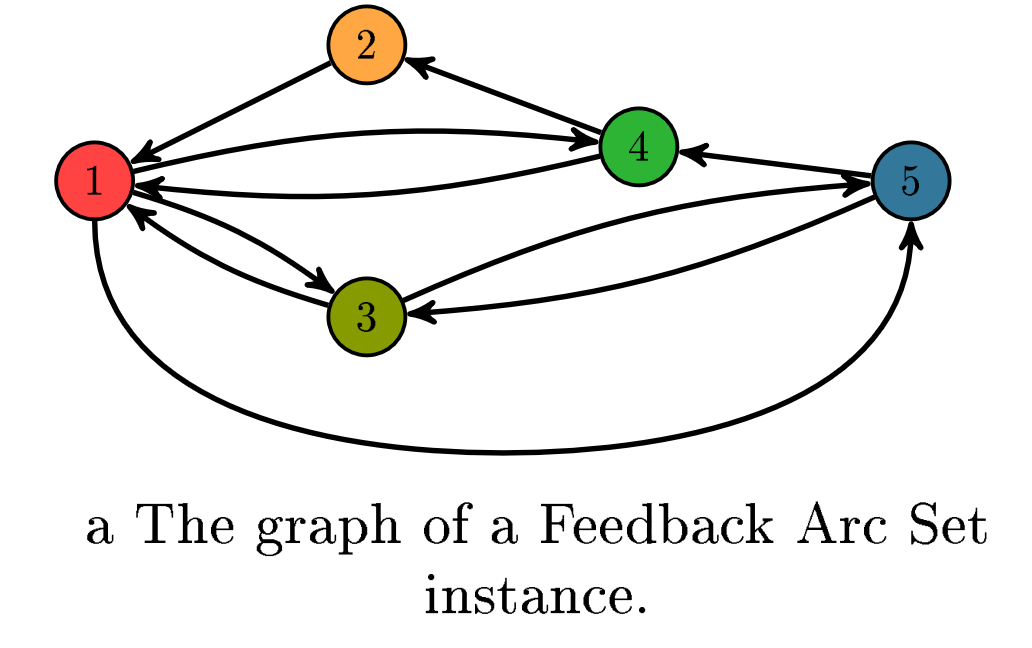
\includegraphics[width=0.75\textwidth]{graph}
    \end{subfigure}%
    \begin{subfigure}{.5\textwidth}
		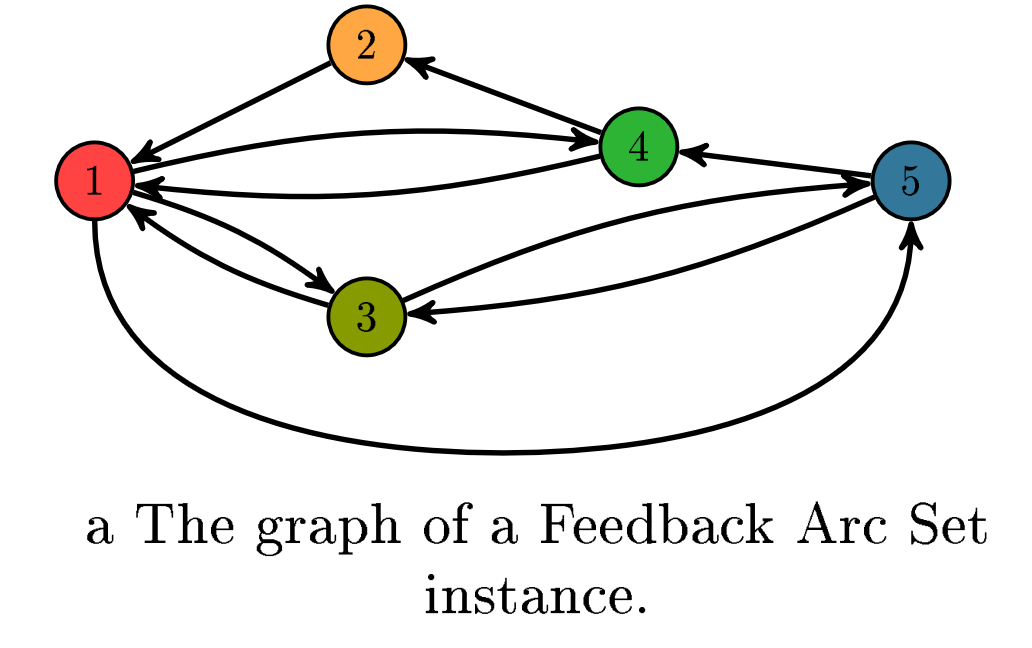
\includegraphics[width=0.75\textwidth]{graph}
    \end{subfigure}
    \caption{Programm für das Verdichtungspuzzle}
	\label{fig:6}
\end{figure}

\newpage

\section{Permutationspuzzle}
Sei eine beschriftete kanonische Ausgangskonfiguration gegeben. Gibt es eine Folge von linepushes, die eine bestimmte Permutation erzeugt? 

\subsection{Selbe Form}
\begin{definition}
Eine beschriftete Konfiguration $K_1$ hat die selbe Form wie eine beschriftete Konfiguration $K_2$, falls die beiden Konfigurationen ohne die Beschriftung der Tokens äquivalent sind.
\end{definition}
\begin{figure}[ht]
	\centering
	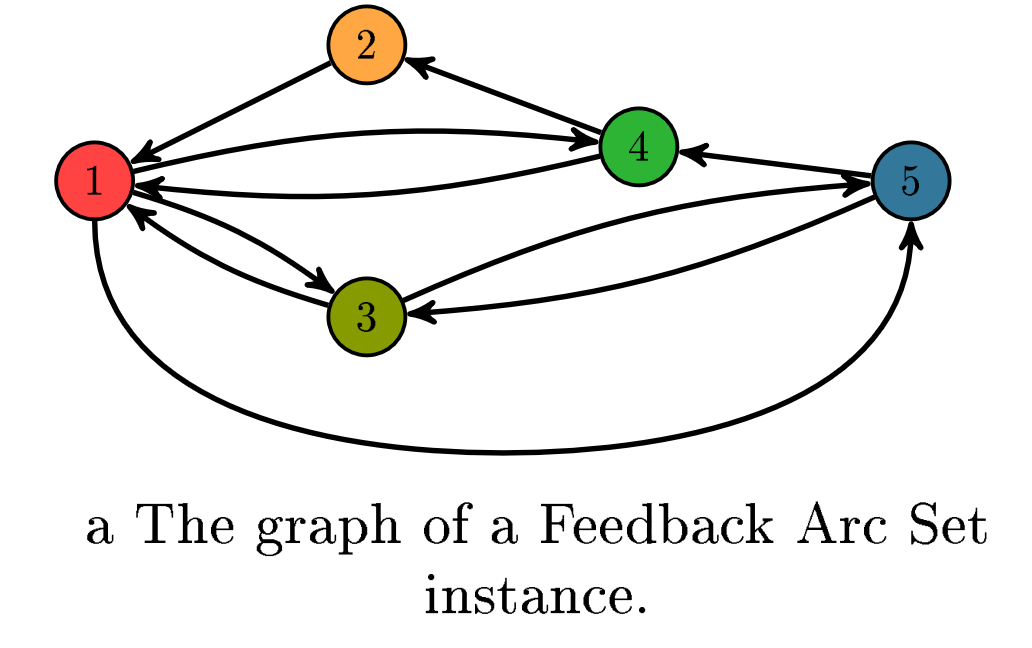
\includegraphics[width=0.7\textwidth]{graph}
	\caption{Konfigurationen der selben Form}
	\quelle \cite{akitaya2022pushing}
	\label{fig:10}
\end{figure}
\noindent Abbildung \ref{fig:10} zeigt zwei Konfigurationen der selben Form mit einer unterschiedlichen Beschriftung. 
\subsection{Permutation}
\begin{definition}
Für die Permutation betrachten wir nur beschriftete kanonische Konfigurationen. Eine Permutation einer beschrifteten Konfiguration ist eine Konfiguration der selben Form.
\end{definition}
\subsection{Dualpuzzle}
Ein Dualpuzzle besteht aus einem Primärpuzzle mit einer kompakten Ausgangskonfiguration und dem Dual. Das Dual wird aus dem Inversen des Primärpuzzles gebildet. Alle leeren Felder im Begrenzungsrechteck des Primärpuzzles werden ausgefüllt und alle gefüllten Felder leer gemacht. Dann werden die Tokens sinnvoll angeordnet, sodass diese eine kompakte Konfiguration bilden. Um diese Konfiguration entsteht schließlich noch ein neues kleineres Begrenzungsrechteck. Ist das Primärpuzzle kanonisch, so nennt man das Dualpuzzle auch kanonisch.

\begin{figure}[ht]
	\centering
	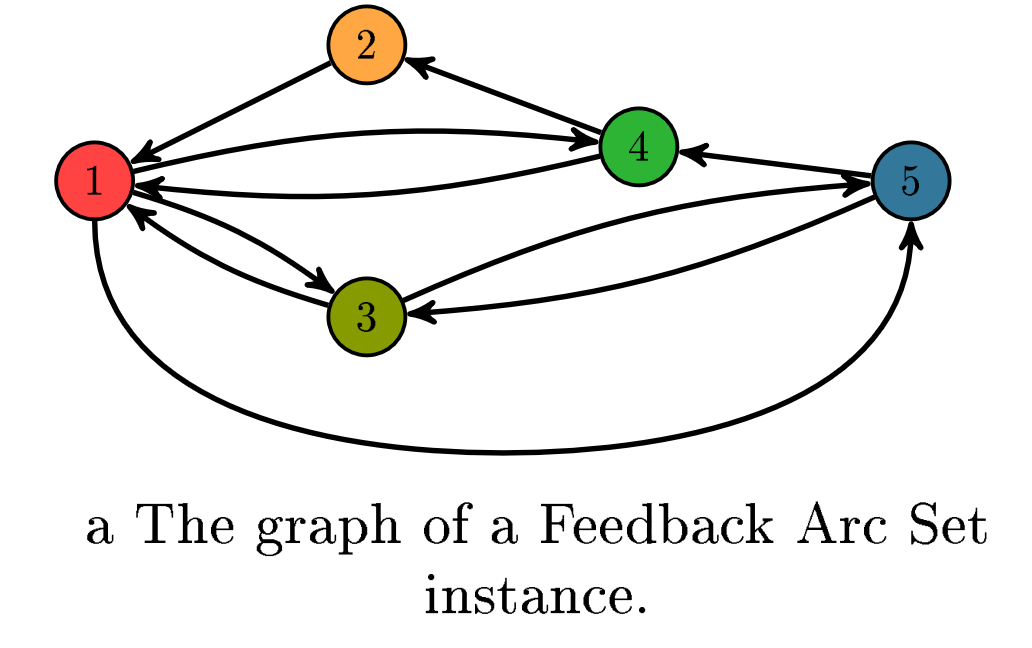
\includegraphics[width=0.5\textwidth]{graph}
	\caption{Primärpuzzle (links) / Dual (rechts)}
	\quelle \cite{akitaya2022pushing}
	\label{fig:11}
\end{figure}

\newpage
\subsection{Unbeweglicher Zentraler Kern}
Bei einem Permutationspuzzle schauen wir uns Permutationen einer Ausgangskonfiguration an. Jedoch sind unter bestimmten Umständen manche Tokens nicht beweglich. Falls mehr als die Hälfte der Reihen und mehr als die Hälfte der Spalten voll ist, so existiert ein unbeweglicher zentraler Kern. Die Tokens in diesem Kern lassen sich durch keinen linepush innerhalb des Begrenzungsrechtecks verschieben.

\begin{figure}[ht]
	\centering
	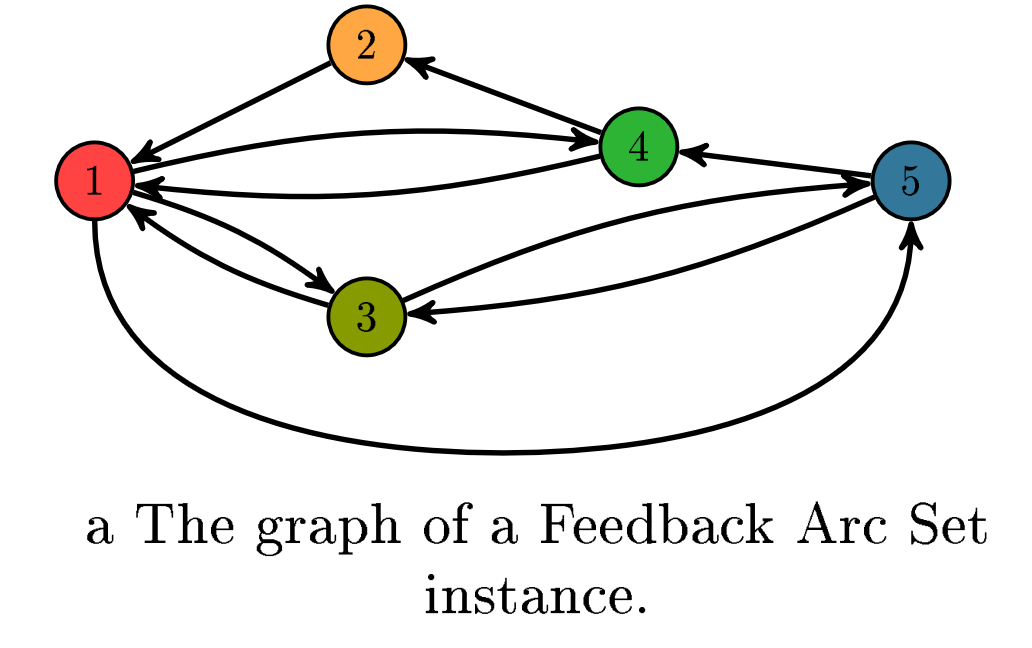
\includegraphics[width=0.29\textwidth]{graph}
	\caption{Konfiguration mit einem unbeweglichen zentralen Kern}
	\quelle \cite{akitaya2022pushing}
	\label{fig:12}
\end{figure}

\noindent Da die doppelte Anzahl ausgefüllter Reihen in Abbildung \ref{fig:12}, also Reihen die von einer Seite des Begrenzungsrechtecks zur anderen Seite reichen, größer als die Anzahl der Reihen ist und dies gleichermaßen für die Spalten gilt, haben wir einen unbeweglichen zentralen Kern. Dieser Kern ist mit einem blauen Rechteck in der Abbildung \ref{fig:12} gekennzeichnet.
\subsection{Theorem}
Alle möglichen Permutationen sind nur mit einer geraden Anzahl von Transpositionen erreichbar. Das heißt alle möglichen Permutationen sind gerade.
\begin{proof}\noindent\\
Zuerst bilden wir das Dual eines Dualpuzzle und erhalten ein Puzzle, das den Regeln eines Primärpuzzles folgt. Das Begrenzungsrechteck des Duals eines Puzzles ist dazu immer kleiner als das Begrenzungsrechteck des Puzzles selber. Daher können wir nun mit Induktion über die Größe des Begrenzungsrechtecks argumentieren.\\\\
Falls das Begrenzungsrechteck ausgefüllt ist, so haben wir nur die Permutation der Identität vorliegen, da linepushes nichts bewirken. Die Identität ist eine gerade Permutation.\\\\
Allgemein gilt für ein Primärpuzzle, dass auf jeden linepush, der eine nicht äquivalente Konfiguration zum Vorherigen erzeugt, ein entgegengesetzter linepush, der auch eine nicht äquivalente Konfiguration erzeugt, innerhalb der Sequenz folgen muss. Denn die Endkonfiguration muss die selbe Form zur Ausgangskonfiguration haben.\\\\
Es sei nun eine nicht verdichtete kanonische Konfiguration $C$ gegeben. Dieses Puzzle bildet ein kanonisches Dualpuzzle. Das Dual des Dualpuzzles ist eine kanonische Konfiguration $D$ mit einem kleineren Begrenzungsrechteck als das von $C$. Durch die kleinere Größe des Begrenzungsrechteck gilt die Induktionshypothese. Nach Durchführung von mehreren linepushes und dem Wiederherstellen von einer kanonischen Konfiguration haben wir nun eine Permutation $\pi$ von $D$  und eine Permutation $\sigma$ von $C$ vorliegen. Da $C$ und $D$ den Regeln des Primärpuzzles folgen, ist die gesamte Permutation $\pi\sigma$ gerade. Durch die Induktionshypothese ist $\sigma$ gerade und daher auch $\pi$.
\end{proof}

\subsection{Generierung von Zyklen}
Alle möglichen Permutationen können mit folgenden Sequenzen erreicht werden. Diese Sequenzen haben die Variable $k\in \mathbb{N}_0$, mit der die unterschiedlichen Permutationen erreicht werden. Die Richtungen in der Sequenz geben dabei die Richtung der linepushes an.
\begin{itemize}
		\item Typ-A $k$-Sequenz: $\langle  \Leftarrow^k~ \Leftarrow ~\Downarrow~ \Rightarrow ~\Uparrow ~\Rightarrow^k ~\rangle$
		\item Typ-B $k$-Sequenz: $\langle \Downarrow^k ~\Downarrow ~\Leftarrow ~\Uparrow~ \Rightarrow ~\Uparrow ^k\rangle$
		\item Typ-C $k$-Sequenz: $\langle \Leftarrow^k~ \Downarrow ~\Leftarrow~ \Uparrow ~\Rightarrow ~ \Rightarrow^k \rangle$
	\end{itemize}
	
\begin{figure}[ht]
	\centering
	\begin{subfigure}{.25\textwidth}
		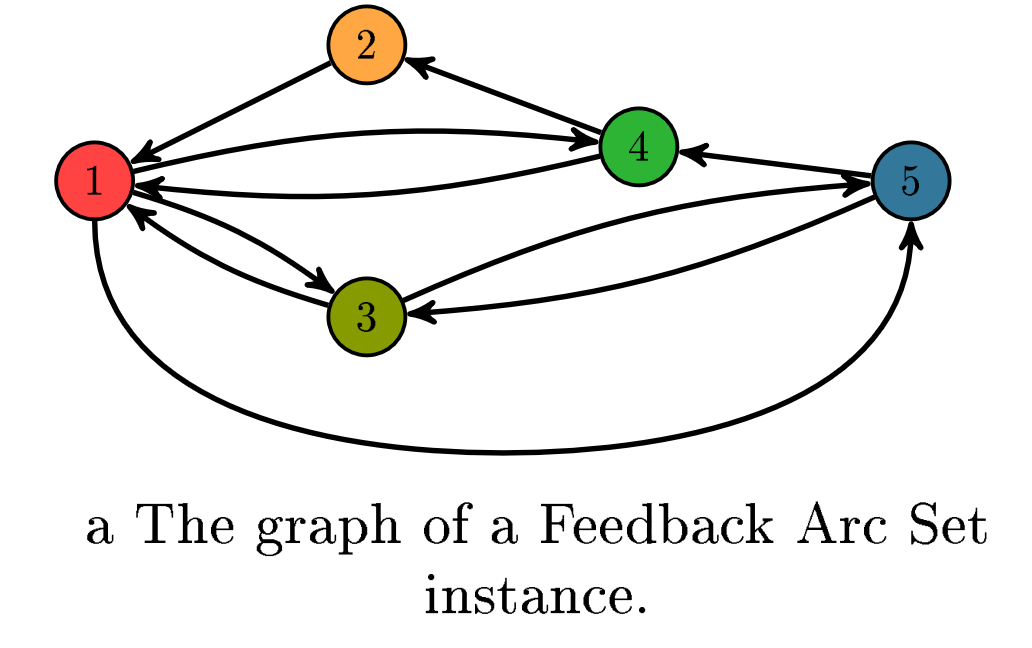
\includegraphics[width=0.75\textwidth]{graph}
    \end{subfigure}%
    \begin{subfigure}{.25\textwidth}
		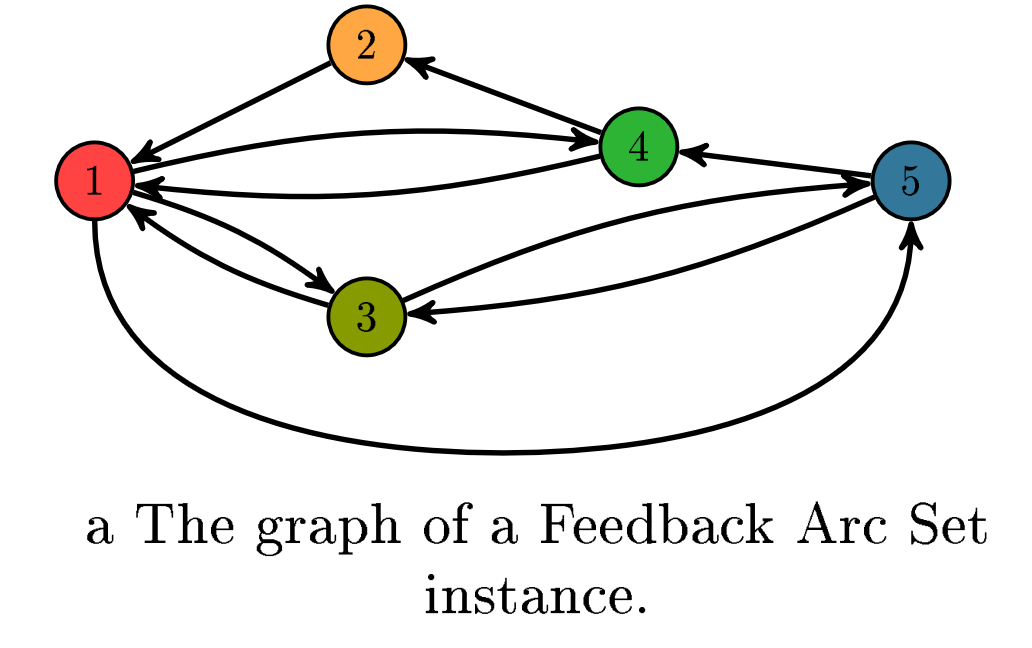
\includegraphics[width=0.75\textwidth]{graph}
    \end{subfigure}
    \caption{Typ-A $4$-Sequenz}
    \quelle \cite{akitaya2022pushing}
	\label{fig:17}
\end{figure}
\newpage
\subsection{Theorem}
Sei $G_C$ unsere Permutationsgruppe für unser Puzzle.\\\\
Falls kein Feld frei ist, dann ist $G_C$ die triviale Gruppe.\\
Das Begrenzungsrechteck ist gefüllt und linepushes verändern die Konfiguration nicht und daher liegt die triviale Gruppe, auch Identität genannt, vor. Dies erkennt man auch in Abbildung \ref{fig:15}.

\begin{figure}[ht]
	\centering
	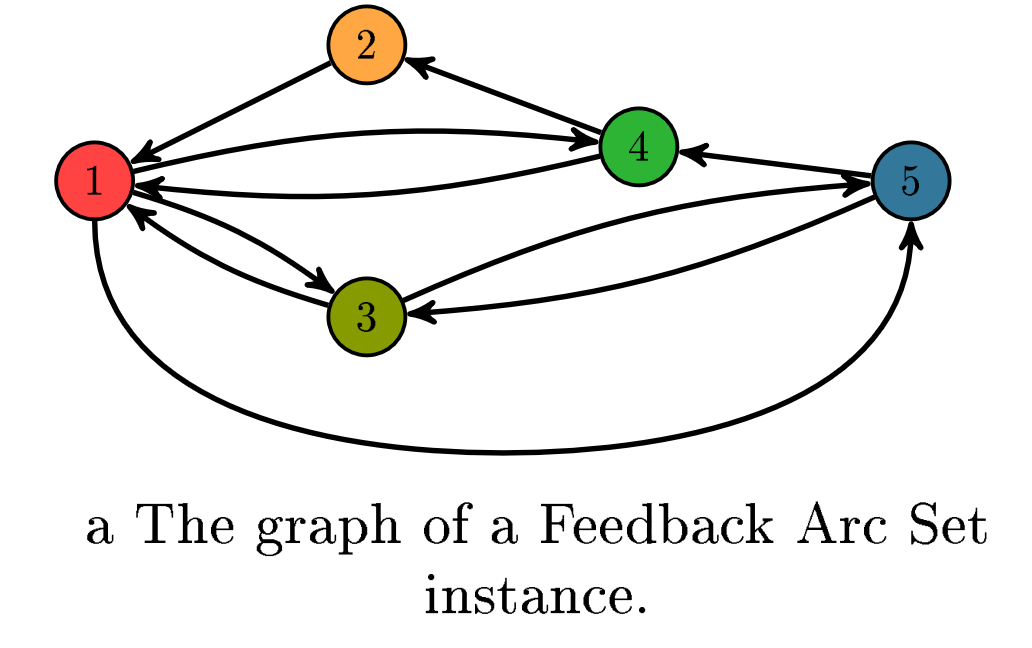
\includegraphics[width=0.23\textwidth]{graph}
	\caption{Dichte Konfiguration}
	\quelle\cite{akitaya2022pushing}
	\label{fig:15}
\end{figure}

\noindent
Falls genau ein Feld frei ist, dann wird $G_C$ zyklisch über die nicht-Kern Tokens generiert, da Permutationen nur durch das zyklische Rotieren der Tokens am Rand des Begrenzungsrechteck möglich sind wie in Abbildung \ref{fig:16} zu sehen ist.

\begin{figure}[ht]
	\centering
	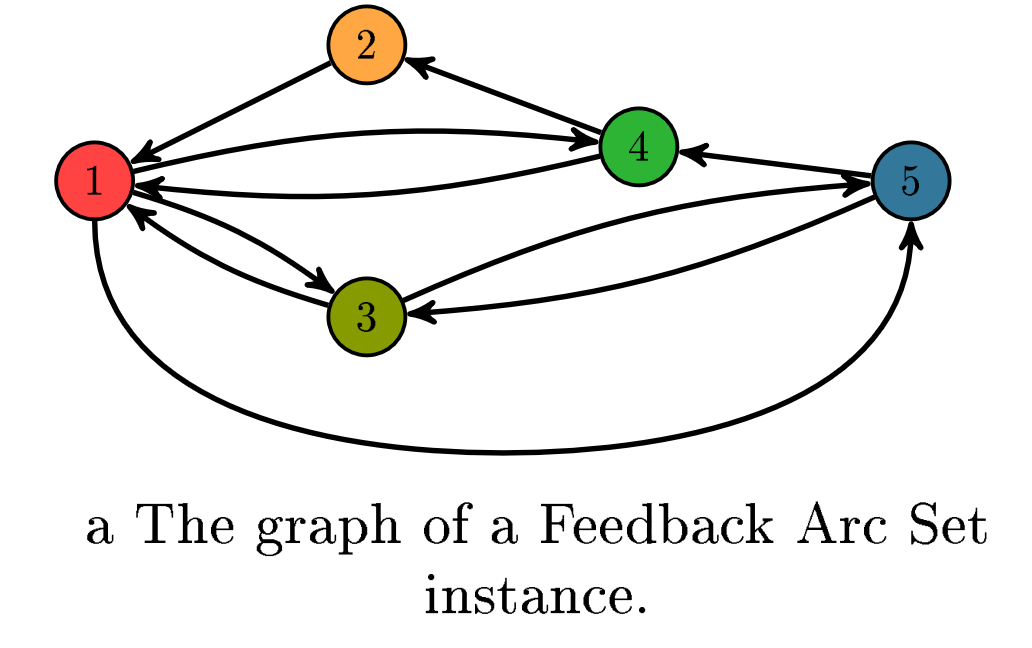
\includegraphics[width=0.23\textwidth]{graph}
	\caption{zyklische Permutation}
	\quelle\cite{akitaya2022pushing}
	\label{fig:16}
\end{figure}

\noindent
Ansonsten ist $G_C$ entweder isomorph zu der alternierenden Gruppe und hat somit eine ähnliche Struktur und Eigenschaften wie diese oder die alternierende Gruppe über die nicht-Kern Tokens. 
Die alternierende Gruppe ist dabei die Permutationsgruppe, die alle geraden Permutationen beinhaltet.

\subsection{Programm}
Für das Permutationspuzzle hab ich ebenso ein JavaFX Programm geschrieben, um mit diesem linepushes zu simulieren und mögliche Permutationen anzuschauen.\\
Hier wird, wie beim Verdichtungspuzzle, ein Raster mit roten beschrifteten Tokens angezeigt und durch das Drücken auf die Knöpfe kann ein linepush in die Richtung des Pfeiles auf den Knöpfen ausgeführt werden. Dazu ist es möglich, die Beschriftung der leeren Felder sich auch anzeigen zu lassen, wie in den oberen beiden Bildern in Abbildung \ref{fig:14} zu sehen ist.\\
 Da wir uns nur kompakte Konfigurationen anschauen, wird hier die Anpassung des Begrenzungsrechtecks nicht benötigt und daher bleibt dieses bei jedem linepush gleich.
\begin{figure}[ht]
	\centering
	\begin{subfigure}{.4\textwidth}
		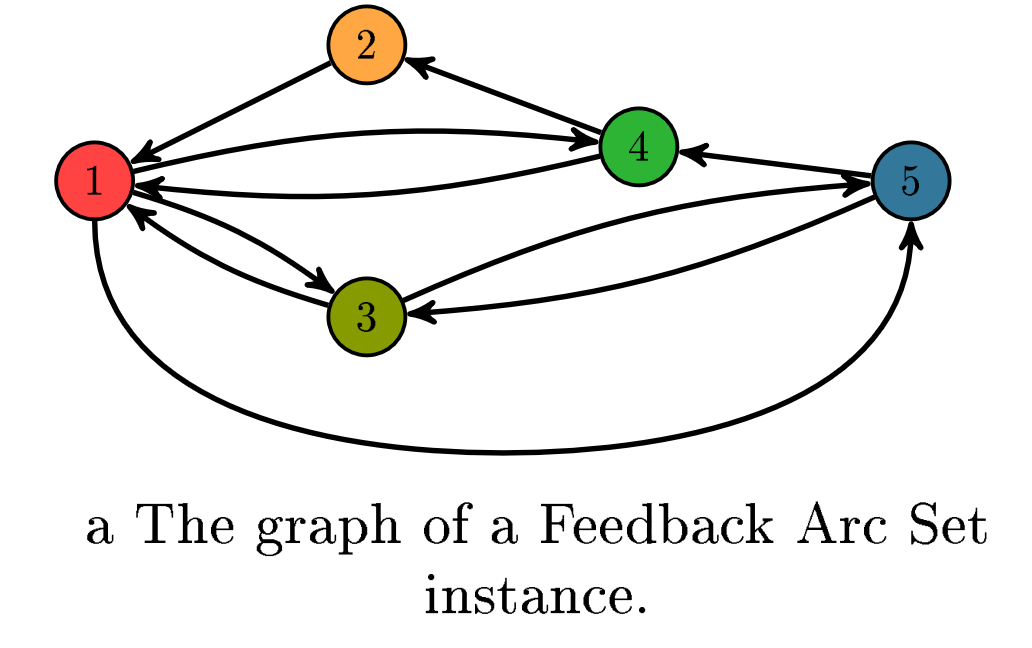
\includegraphics[width=0.78\textwidth]{graph}
    \end{subfigure}%
    \begin{subfigure}{.4\textwidth}
		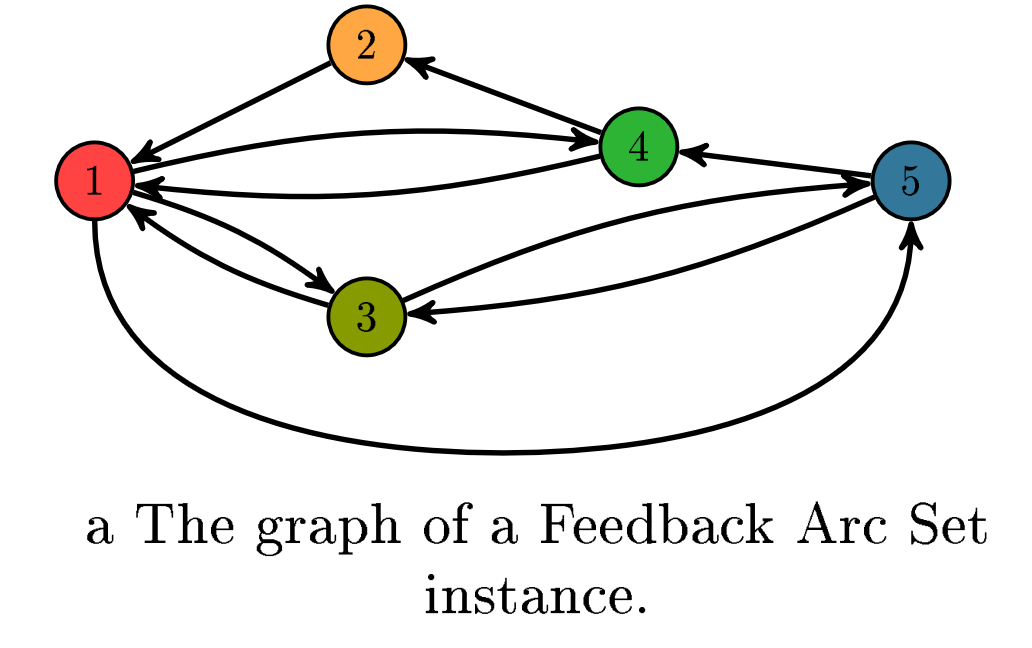
\includegraphics[width=0.78\textwidth]{graph}
    \end{subfigure}
\end{figure}
\begin{figure}[ht]
	\centering
	\begin{subfigure}{.4\textwidth}
		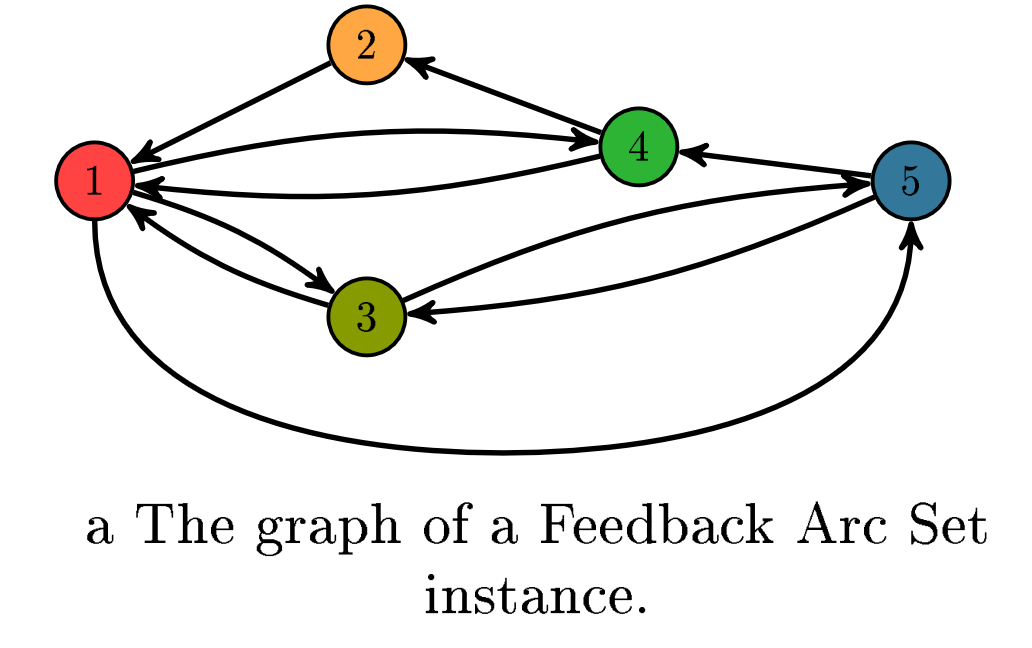
\includegraphics[width=0.78\textwidth]{graph}
    \end{subfigure}%
    \begin{subfigure}{.4\textwidth}
		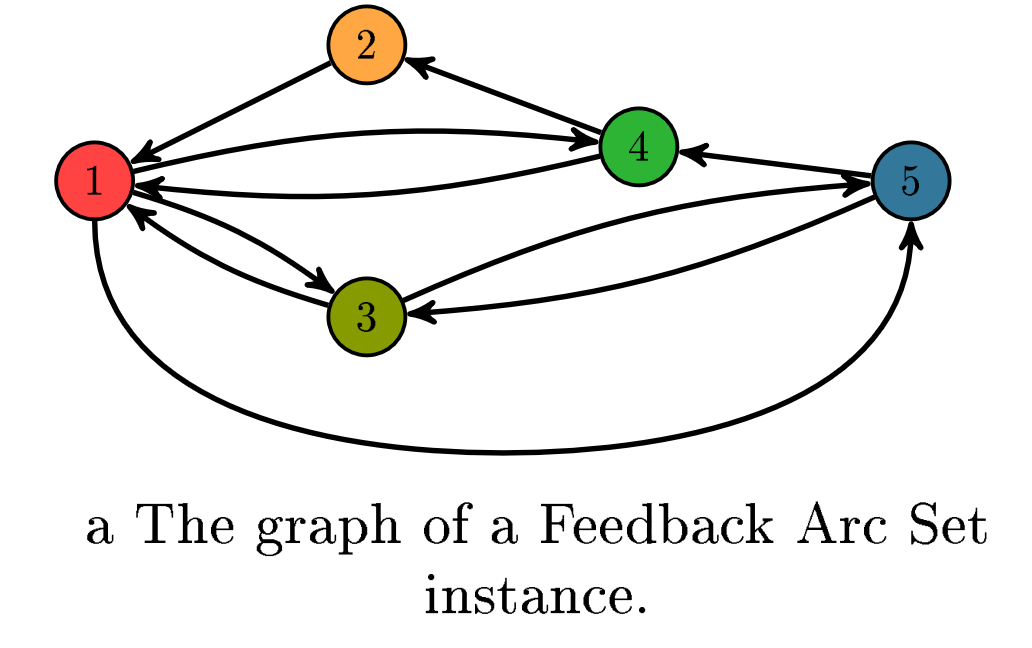
\includegraphics[width=0.78\textwidth]{graph}
    \end{subfigure}
\end{figure}
\begin{figure}[ht]
	\centering
	\begin{subfigure}{.4\textwidth}
		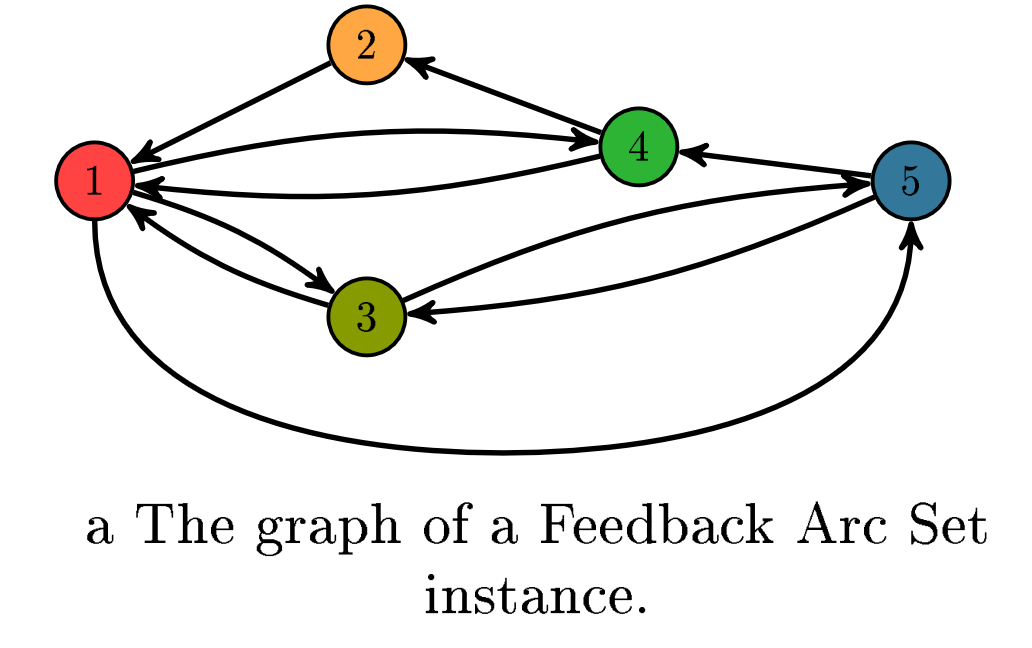
\includegraphics[width=0.78\textwidth]{graph}
    \end{subfigure}%
    \begin{subfigure}{.4\textwidth}
		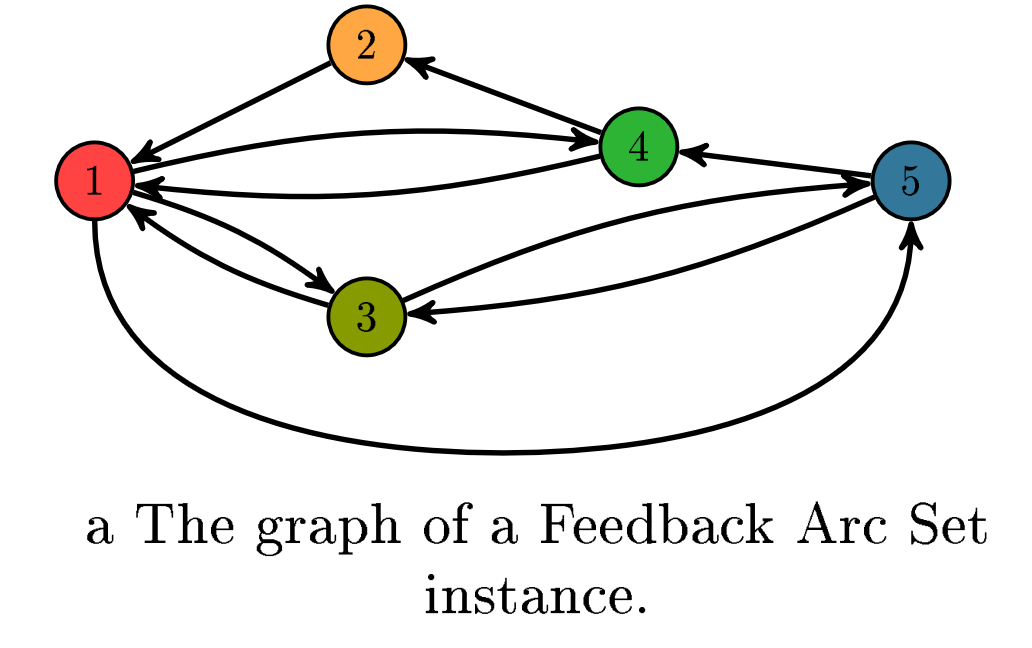
\includegraphics[width=0.78\textwidth]{graph}
    \end{subfigure}
    \caption{Programm für das Permutationspuzzle}
	\label{fig:14}
\end{figure}
\newpage
\noindent Auch für das Dualpuzzle habe ich ein JavaFX Programm geschrieben. Dieses gleicht der Funktionsweise des Permutationspuzzles, aber dazu wird eine weitere GridPane angezeigt, auf der das zum Primärpuzzle entsprechende Dual abgebildet ist. Die für das Dual gespeicherten Werte werden folgenden berrechnet: Im ersten Schritt werden die inversen Werte zum Primärpuzzle gebildet. Dies bedeutet, dass jede \glqq$1$\grqq{}  aus dem Primärpuzzle zur \glqq$0$\grqq{} im Dual wird und die \glqq$0$\grqq{} zur \glqq$1$\grqq{}. Die \glqq$0$\grqq{} zeigt dabei ein Rasterfeld ohne Token und die \glqq$1$\grqq{} ein Rasterfeld mit einem Token an. Im zweiten Schritt werden die Tokens durch Verschiebungen zu einer kompakten Konfiguration geformt und schließlich wird ein berechnetes blaues Begrenzungsrechteck für das Dual hinzugefügt.
\begin{figure}[ht]
	\centering
	\begin{subfigure}{.4\textwidth}
		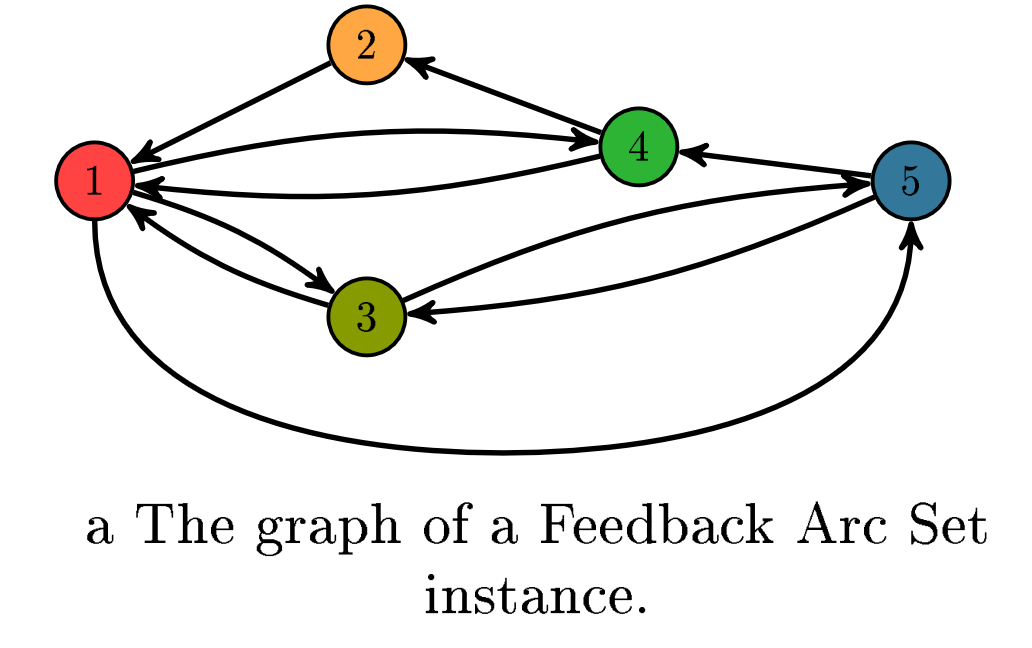
\includegraphics[width=0.9\textwidth]{graph}
    \end{subfigure}%
    \begin{subfigure}{.4\textwidth}
		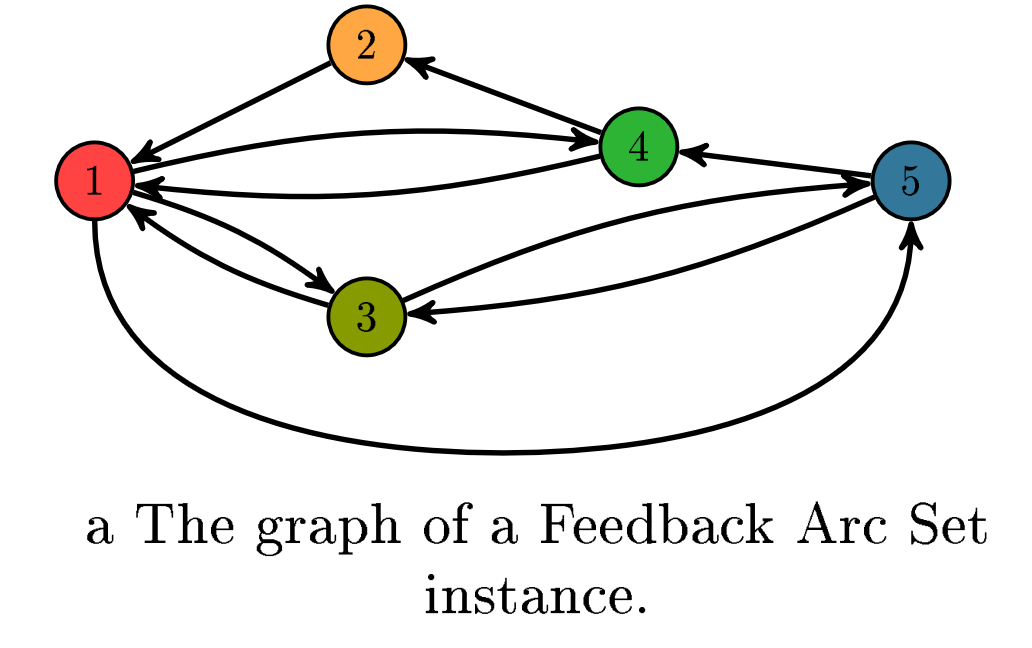
\includegraphics[width=0.9\textwidth]{graph}
    \end{subfigure}
    \caption{Programm für das Dualpuzzle}
	\label{fig:6}
\end{figure}





%%%%%%%%%%%%%%%%%%%%%%%%%%%%%%%%%%%%%%%%%%%%%%%%%%%%%%%%%%%%%%%%%%%%%%%%%%%%%%%%
\clearpage
\nocite{*}
\printbibliography


\end{document}
